\documentclass[12pt,a4paper]{article}
\usepackage[utf8]{vietnam}
\usepackage{amsmath}
\usepackage{amsfonts}
\usepackage{amssymb}
\usepackage{array}
\usepackage[left=2cm,right=2cm,top=2cm,bottom=2cm]{geometry}
\author{Huu Tai}
\usepackage{indentfirst}
\usepackage{footnote}
\usepackage{graphicx}
\usepackage{listings}
\usepackage{scrextend}
\changefontsizes{13pt}
\begin{document}
\section{Vấn đề về đánh giá tự động cho bài tập lập trình}
\subsection{Giới thiệu}
Trong thời kỳ ngày càng phát triển của mạng internet thì việc chấm điểm tự động cho các bài tập lập trình ngày càng trở nên quan trọng hơn đặc biệt là khi có sự xuất hiện của các khóa học trực tuyến ngày càng phổ biến hoặc là các lớp học có sinh viên tham gia với số lượng lớn. Đánh giá là một phần không thể thiếu trong giáo dục và thường được sử dụng để đánh giá và cung cấp kết quả cho sinh viên tham gia vào môn học. Đồng thời dựa vào các kết quả đánh giá sau môn học của sinh viên mà giáo viên có thể xác định liệu chương trình giảng dạy có đáp ứng được nhu cầu cần thiết của sinh viên hay không.

\indent Trong lĩnh vực giáo dục tâm lý, người ta đã chứng minh rằng hầu hết sinh viên thường hướng những nỗ lực của họ dựa trên kết quả của các bài kiểm tra sau khi được đánh giá và ảnh hưởng của các kết quả đó đến kết quả cuối cùng của khóa học. Đánh giá liên tục trong một khóa học lập trình đảm bảo rằng sinh viên hoàn thành đủ các bài kiểm tra cũng như nhận lại phản hồi về kết quả của các bài kiểm tra đó. Tuy nhiên việc đánh giá kết quả một cách thủ công cho một lớp học đòi hỏi rất nhiều công sức và rất dễ bị lỗi và việc đấy càng được thể hiện rõ ràng khi số lượng sinh viên trong một lớp học tăng lên (Ví dụ, các khóa học lập trình khác nhau trên edX plat-form có hơn 150000 sinh viên đăng ký trên toàn thế giới \cite{liu2019automatic}), điều đó làm cho việc chấm điểm nhanh chóng cho tất cả các bài tập của sinh viên trở nên khó khăn hơn nhiều. Nhiều khóa học trực tuyến áp dụng phản hồi ngang hàng \cite{weld2012personalized}, nhưng loại phản hồi này không đáp ứng được như mong muốn. Sinh viên phải chờ hàng giờ để nhận được phản hồi và giáo viên hướng dẫn chỉ có kiến thức hạn chế về các quy trình đánh giá ngang hàng không có cấu trúc này. Lúc đó việc đánh giá kết quả của sinh viên đòi hỏi phải được giới hạn hoặc hợp lý hóa theo một cách nào đó.

\indent Trong thực tế hai giáo viên chấm cùng một môn rất hiếm khi áp dụng cùng một tiêu chí đánh giá trong mọi trường hợp. Điều này là không công bằng với sinh viên bởi vì điều đó có nghĩa là điểm đánh giá của học sinh có thể phụ thuộc vào từng giải pháp đánh giá của giáo viên mà không chỉ dựa vào giải pháp của học sinh. Và việc này càng xảy ra phổ biến trong việc đánh giá các bài tập lập trình.

\indent Thông thường sẽ có vô số giải pháp khả thi cho cùng một vấn đề vì có thể có thể có các biến thể trong các bài tập lập trình do đó một mẫu đánh giá sẽ cũng cấp hướng dẫn cho người đánh giá nhưng sẽ không bao quát hết tất các cả trường hợp. Điều đó đòi hỏi phải có một công cụ giúp đánh giá các bài kiểm tra một cách tự động và hơn hết là đảm bảo đánh giá một cách công bằng, khách quan và được áp dụng như nhau cho tất cả học sinh. Thách thức này đã dẫn đến sự phát triển của các công cụ chấm điểm tự động.

\indent Hiện nay đã có nhiều hệ thống đánh giá tự động tồn tại nhưng hàng năm vẫn có rất nhiều hệ thống đánh giá khác được tạo ra. Các hệ thống đã tồn tại đều đã đáp ứng hầu hết các nhu cầu về đánh giá.
Một lý do rõ ràng cho sự đa dạng của các công cự đó là tuổi thọ và tính khả dụng của nó. Các công cụ đánh giá được tạo ra như là một phần của các khóa học. Nó giúp cho việc đánh giá kết quả của toàn bộ học viên trong khóa học một cách nhanh chóng nhưng không phù hợp để phân phối rộng rãi cho các khóa học khác. Thông thường các công cụ được các giảng viên sử dụng để hỗ trợ trong việc đánh giá các bài tập lập trình vì vậy rất ít các công cụ xuất hiện dưới dạng phần mềm được hỗ trợ và sử dụng rộng rãi. Vì vậy các các công cụ đánh giá tự động thường được lặp đi lặp lại rất nhiều đồng thời có rất ít các công cụ đánh giá tự động được sử dụng một cách rộng rãi và phổ biến.

\indent  Trong bài báo cáo này sẽ trình bày và so sánh các công cụ được sử dụng để chấm điểm tự động cho các bài tập lập trình.

\subsection{Các lỗi phần mềm}
Trước khi trình bày về các kỹ thuật và hệ thống tự động đánh giá tôi muốn giới thiệu các lỗi thường được xem xét đến bởi các kỹ thuật này. Lỗi phần mềm được định nghĩa là tạo ra kết quả sai hoặc thực hiện một hành động theo cách không lường trước được. Lỗi phần mềm được phân loại thành các lỗi như: Lỗi cú pháp, lỗi logic và lỗi thời gian chạy.

\begin{itemize}
\item[-] \textbf{Lỗi cú pháp}: Lỗi này được phát hiện khi cú pháp không chính xác trong ngôn ngữ lập trình, ví dụ như cấu trúc chương trình không chính xác, các từ sai, thiếu dấu chấm phẩy. Loại lỗi này có thể được trình biên dịch ngôn ngữ lập trình phát hiện trong khi biên dịch mã phần mềm. Lỗi này là lỗi dễ phát hiện và sửa nhất vì hầu hết các trình biên dịch được sử dụng ngày nay như GCC hoặc JRE đều cung cấp mô tả đầy đủ về lỗi.
\item[-] \textbf{Lỗi logic}: Khi mắc lỗi này phần mềm biên dịch vẫn chạy tốt nhưng đầu ra của phần mềm bị sai do nhiều lý do như sai về yêu cầu hoặc đặc tả, lỗi toán học (chia cho 0). Vì lỗi này không được trình biên dịch phát hiện nên ta cần phát hiện các lỗi này trước khi khởi chạy phần mềm.
\item[-] \textbf{Lỗi thời gian chạy}: Đây là lỗi nâng cao và rất hiếm khi sinh viên bị rơi vào. Lỗi thời gian chạy chỉ xảy ra khi phần mềm đang chạy. Trong thực tế đây là một trong những vấn đề phức tạp nhất để theo dõi và dẫn đến sự cố phần mềm.
\end{itemize}
\subsection{Lợi ích của việc sử dụng đánh giá tự động}
Việc áp dụng các hệ thống tự động đánh giá vào trong các khóa học đem lại các lợi ích sau:

\begin{itemize}
\item[-] \textbf{Tốc độ}: Giúp cho việc đánh giá nhanh hơn nhiều và sinh viên sẽ nhận được kết quả ngay sau kỳ thi. Khi sử dụng đánh giá thủ công thì sinh viên cần chờ một khoảng thời gian rất lâu để nhận được kết quả đánh giá của bài kiểm tra. Ngược lại với hệ thống đánh giá tự động, các sinh viên có thể tự đánh giá bài kiểm tra của mình, biết điểm của họ và sửa lỗi của chính họ.
\item[-] \textbf{Công bằng}: Các lỗi tương tự sẽ được đánh giá như nhau và giáo viên sẽ không ảnh hưởng đến việc chấm điểm.
\item[-] \textbf{Độc lập}: Việc đánh giá một bài kiểm tra không bị ảnh hưởng từ kết quả của các bài kiểm tra trước đó. Trong đánh giá thủ công, một bài kiểm tra lúc trước có kết quả không tốt có thể khiến giáo viên chủ quan coi bài kiểm tra tiếp theo là không tốt.
\end{itemize}

\section{Kỹ thuật sử dụng trong các hệ thống đánh giá tự động và các công cụ}
Hiện nay có rất nhiều hệ thống đánh giá tự động đang tồn tại nhưng để đảm bảo rằng các hệ thống đó đem lại kết quả đánh giá một cách chính xác là một điều khó khăn. Một trong những vấn đề quan trọng ảnh hưởng đến kết quả đánh giá của một hệ thống đó là việc xây dựng các bộ kiểm thử có chất lượng cao. Trên thực tế, việc cung cấp các bộ kiểm thử bằng cách thủ công là một quá trình rất chậm và tốn thời gian, điều này dẫn đến việc tạo ra các bộ kiểm thử không hiệu quả và không đầy đủ. Điều này dẫn đến chất lượng của hệ thống đánh giá bị ảnh hưởng.

\indent Công cụ tạo bộ kiểm thử tự động ra đời để giải quyết vấn đề nói trên. Với việc tự động sinh ra các bộ kiểm thử có độ bao phủ cao với các tiêu chí kiểm thử nhằm phát hiện các lỗi sâu trong các hệ thống phần mêm phức tạp, công cụ này đã giúp cải thiện độ chính xác cao của các hệ thống đánh giá tự động. Symbolic execution là một trong các kỹ thuật nổi tiếng được sử dụng trong các công cụ tự động sinh bộ kiểm thử. Trong phần tiếp theo chúng ta sẽ tìm hiểu kỹ hơn về kỹ thuật này và một số công cụ hỗ trợ việc tự động sinh bộ kiểm thử.

\subsection{Symbolic execution}
\subsubsection{Giới thiệu}
Trong hoạt động kiểm thử phần mềm, các ca kiểm thử thường được tạo ra một cách thủ công, gây tốn kém về chi phí cũng như thời gian để hoàn thành công đoạn này. Thực thi tượng trưng (Symbolic execution) được biết đến là một kỹ thuật nổi tiếng với khả năng tự động sinh những bộ test case có độ bao phủ cao với các tiêu chí kiểm thử nhằm phát hiện những lỗi sâu trong các hệ thống phần mềm phức tạp.

\indent Hiện nay có rất nhiều công cụ nền tảng phục vụ cho hoạt động kiểm thử phần mềm như JUnit cho ngôn ngữ Java, Nunit, VSUnit cho .NET để thực thi các ca kiểm thử ở mức đơn vị. Tuy nhiên các công cụ kiểm thử này không hỗ trợ việc sinh tự động các ca kiểm thử đơn vị. Viết các ca kiểm thử là một công việc nặng nhọc và tốn nhiều công sức. Có nhiều phương pháp khác nhau hỗ trợ việc sinh tự động các ca kiểm thử (Test case) giúp giảm chi phí và thời gian thực hiện đã được nghiên cứu và đưa ra như: Dựa trên mô hình (Model Checking), kiểm thử ngẫu nhiên (Random Testing \cite{boyer1975select}). Nhưng hạn chế của nó là kiểm tra cùng 1 hành vị thực thi của chương trình nhiều lần với những đầu vào khác nhau và chỉ có thể kiểm tra được một số trường hợp thực thi của chương trình. Thêm vào đó, kiểm thử ngẫu nhiên khó xác định được khi nào việc kiểm thử nên được dừng lại và nó không biết tại điểm nào không gian trạng thái đã được thám hiểm hết. Để xác định khi nào việc kiểm thử dừng lại thì hệ thống kiểm thử ngẫu nhiên được kết hợp với các tiêu chuẩn an toàn \cite{zhu1997software}. Để khắc phục những hạn chế của kiểm thử ngẫu nhiên, phương pháp thực thi tượng trưng xây dựng các ràng buộc trên các giá trị tượng trưng và giải các ràng buộc đó để sinh ra các giá trị đầu vào cho chương trình mà nó có thể bao phủ tất cả các dòng lệnh cũng như các nhánh thực thi của chương trình.

\indent Ý tưởng của thực thi tượng trưng đã được đề xuất bởi King [Comm. ACM 1976], Clarke [IEEE TSE 1976] nhưng việc hiện thực ý tưởng mới chỉ được thực hiện trong những năm gần đây qua tiến bộ đáng kể trong lý thuyết giải các ràng buộc (Constrain satisfiability) \cite{de2011satisfiability} và các tiếp cận mở rộng thực thi tượng trưng động (Dynamic symbolic execution), một kỹ thuật kết hợp giữa các giá trị cụ thể và giá trị 
tượng trưng cho các giá trị đầu vào.

\subsubsection{Tổng quan về kỹ thuật Symbolic execution}
Ý tưởng chính của Symbolic execution là thực thi chương trình với các giá trị tượng trưng (Symbolic value) thay vì các giá trị cụ thể (concrete value) của các tham số đầu vào. Kết quả là giá trị đầu ra được tính toán bởi chương trình và được biểu diễn bởi bởi một biểu thức tượng trưng. Trong kiểm thử phần mềm, kỹ thuật Symbolic execution được sử dụng để sinh dữ liệu kiểm thử cho mỗi đường thực thi khác nhau của chương trình. Ví dụ trong hình \ref{refhinh1} (trang \pageref{refhinh1}) minh họa cho Symbolic execution.

\indent Trong quá trình thực thi tượng trưng, việc đi theo một nhánh cụ thể nào đó không phụ thuộc vào các giá trị của các tham số đầu vào. Tại tất cả các điểm rẽ nhánh, tất cả các nhánh sẽ được xem xét và kiểm tra nhằm định hướng cho thực thi tiếp theo của chương trình. Với những chương trình ở dạng đơn giản có hại loại thực thi chủ yếu: đó là câu lệnh gán và câu lệnh rẽ nhánh. Tại các câu lệnh gán, giá trị tượng trưng của biến chương trình cũng như các tham số đầu vào có liên quan đến câu lệnh đó được tính toán và cập nhập lại, còn tại các điểm rẽ nhánh, chương trình sẽ điều khiển thực thi theo cả hai nhánh tương ứng đồng thời ràng buộc đường đi (Path condition) tương ứng với hai nhánh sẽ được tạo ra. Một ràng buộc là một biểu thức điều kiện tương ứng với giá trị true, ràng buộc kia tương ứng với giá trị false của biểu thức ràng buộc. Các ràng buộc này sẽ được cập nhập vào đường đi tương ứng với nhánh đó. Các ràng buộc này sẽ được xen xét bởi một bộ giải ràng buộc để đánh giá xem đường đi tiếp theo có khả thi không hay nói một cách khác là kiểm tra xem có tồn tại bộ giá trị thõa mãn ràng buộc này hay không. Nếu không thõa màn thì ràng buộc sẽ đánh giá là sai, khi đó Symbolic execution sẽ dừng hoặc quay lui thực thi theo nhánh khả thi.

\begin{figure}[ht]
\begin{center}
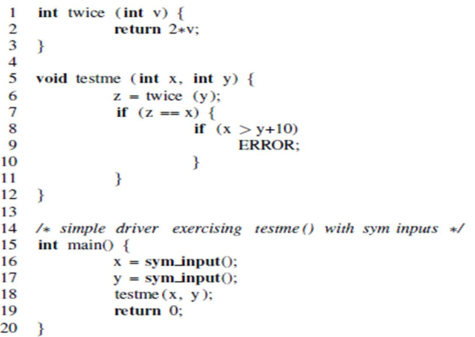
\includegraphics{hinhanh/hinh1}
\end{center}
\caption{Ví dụ cho symbolic execution}
\label{refhinh1}
\end{figure}

\indent Các ràng buộc đường đi được tạo ra bằng cách thu gom các điều kiện trên đường đi tương ứng. Giải các ràng buộc này sẽ sinh ra các giá trị cụ thể cho các tham số đầu vào tương ứng với từng nhánh thực thi của chương trình.

\indent Tất cả các đường thực thi của chương trình có thể biểu diễn bởi một cấu trúc cây gọi là cây thực thi (Tree execution). Hình \ref{refhinh2} (trang \pageref{refhinh2}) là cây thực thi tượng trưng cho hàm testme() trong hình \ref{refhinh1} (trang \pageref{refhinh1}). Các cạnh của cây biểu diễn cho sự chuyển đổi từ trạng thái này sang trạng thái khác. Với ví dụ trên phương thức testme() trong hình \ref{refhinh1} (trang \pageref{refhinh1}) sẽ có cây thực thi mô tả những đường thực thi của chương trình với các biến đầu vào là {x=0, y=1}, {x=2, y=1}, {x=30, y=15}, mục tiêu là sinh ra tập các ca kiểm thử thõa mãn thực thi cho tất cả các nhánh của chương trình phụ thuộc vào giá trị tượng trưng của các tham biến đầu vào nhiều nhất có thể trong một khoảng thời gian nhất định đảm báo khám phá chính xác tất cả các đường thực thi bởi một lần duy nhất với những giá trị đầu vào đã cho.

\begin{figure}[ht]
\begin{center}
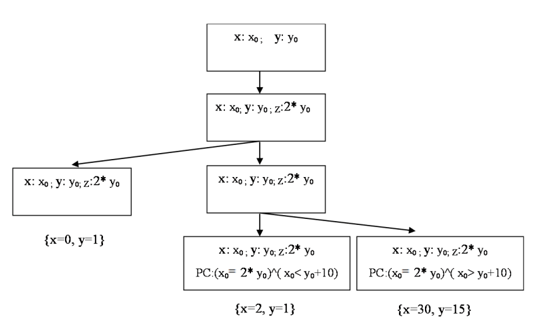
\includegraphics{hinhanh/hinh2}
\end{center}
\caption{Cây Symbolic execution tương ứng với hàm testme() trong ví dụ 1}
\label{refhinh2}
\end{figure}

\indent Bắt đầu thực thi tượng trưng hàm testme() bằng việc gán giá trị cho các tham số đầu vào x và y lần lượt là $x_0$, $y_0$. Khởi tạo PC (Path condition) nhận giá trị là true, tới câu lệnh rẽ nhánh $if(2*y_0=x_0)$ hai nhanh của chương trình tương ứng đều được thực thi với các giá trị tương ứng là $x_0$ và $y_0$. Tại đây biểu thức điều kiện rẽ nhánh là $2*y_0=x_0$ và $!(2*y_0=x_0)$ được bổ sung và PC theo hai nhánh khác nhau. Sau khi thực thi câu lệnh $if(2*y_0=x_0)$ hàm testme() được thực thi theo nhánh mà tồn tại bộ giá trị x,y thõa mãn. Tương tự như trên, khi gặp câu lệnh $if(x_0>y_0+10)$ PC theo hai nhánh tương ứng sẽ được cập nhập bổ sung là $(2*y_0=x_0)$ \^{} $(x_0>y_0+10)$ và $(2*y_0=x_0)$\^{}$(x_0<y_0+10)$. Tại mỗi điểm rẽ nhánh PC sẽ được cập nhập và một thủ tục quyết định bằng bộ xử lý ràng buộc sẽ được sử dụng để xác định xem nhánh tương ứng với PC đó có khả thi hay không để điều hướng thực thi hiện thời đi theo nhánh đó. Nếu PC được đánh giá là không khả thi thực thi tượng trưng sẽ dừng hoặc quay lui, và thực thi tượng trưng chỉ thực thi chương trình tượng trưng theo nhánh mà PC được đánh giá là khả thi.

\indent Đối với những đoạn mã chứa vòng lặp hoặc lời gọi đệ quy mà đường thực thi là vô hạn và biến điều khiển của vòng lặp hoặc lời gọi đệ quy là tượng trưng. Ví dụ trong hình \ref{refhinh3} (trang \pageref{refhinh3}) sẽ là vô hạn đường thực thi với mỗi đường thực thi là 1 dãy tùy ý số lượng giá trị là true và sau cùng là false hoặc là một dãy vô hạn số lần lặp, khi đó PC của đường thực thị là một dãy gồm n giá trị true và sau cùng là false.

\begin{figure}[ht]
\begin{center}
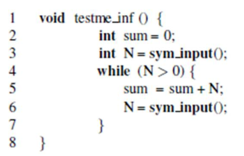
\includegraphics{hinhanh/hinh3}
\end{center}
\caption{Ví dụ cho vòng lặp vô hạn}
\label{refhinh3}
\end{figure}

\indent Trên thực tế cần phải thêm các tiêu chí giới hạn cho việc tìm kiếm như thời gian thực thi, giới hạn chiều sâu của đường thực thi hoặc số lượng các vòng lặp lồng nhau.

\indent Nhược điểm chính của Symbolic execution truyền thống là không thể sinh dữ liệu test nếu không giải được biểu thức ràng buộc đường thực thi. Ví dụ nếu ta thay hàm twice() ở hình \ref{refhinh1} (trang \pageref{refhinh1}) bằng hàm twice() ở hình \ref{refhinh4} (trang \pageref{refhinh4}) sau khi thực hiện câu lệnh dòng 7 thì thực thi tượng trưng sẽ cho ra hai ràng buộc mới bổ sung $x_0$\#$y_0$*$y_0$\%50 và $x_0=y_0$*$y_0$\%$50$ và khi bộ giải ràng buộc không giải được ràng buộc trên thực thi tượng trưng sẽ thất bại trong việc sinh các dữ liệu kiểm thử cho chương trình sau khi đã được sửa đổi.

\begin{figure}[ht]
\begin{center}
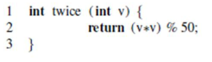
\includegraphics{hinhanh/hinh4}
\end{center}
\caption{Ví dụ cho hàm twice()}
\label{refhinh4}
\end{figure}

\subsubsection{Các kỹ thuật Symbolic execution hiện đại}

Một trong những yếu tố quan trọng của kỹ thuật thực thi tượng trưng hiện đại là khả năng kết hợp giữa giá trị cụ thể và giá trị tượng trưng. Chúng tôi sẽ trình bày dưới đây hai kỹ thuât quan trọng và đánh giá những ưu điềm mà các kỹ thuật này cung cấp.

\begin{enumerate}
\item \textbf{Concolic testing}

Directed Automated Random Testing (DART) \cite{ganesh2007decision} thực hiện kỹ thuật tượng trưng động (là kỹ thuật phân tích chương trình động). Thực thi tượng trưng động chính là sự kết hợp giữa thực thi cụ thể và thực thi tượng trưng. Trong thực thi tượng trưng động, chương trình được thực thi nhiều lần với những giá trị khác nhau của tham số đầu vào.

Bắt đầu bằng việc chọn những giá trị tùy ý cho các tham số đầu vào và thực thi chương trình với những giá trị cụ thể đó chương trình sẽ được thực thi theo một đường đi xác định. DART thực thi chương trình với các giá trị cụ thể của tham số đầu vào và thu gom các ràng buộc trong quá trình thực thi theo đường đi mà sự thực thi cụ thể này đi theo, đồng thời suy ra các ràng buộc mới từ những ràng buộc đã thu gom được.

Tại các câu lệnh rẽ nhánh, biểu thức điều kiện rẽ nhánh sẽ được đánh giá theo các giá trị cụ thể của các tham số đầu vào. Nếu biểu thức điều kiện rẽ nhánh nhận giá trị là True thì biểu thức của điều kiện rẽ nhánh sẽ được thu gom vào ràng buộc của PC và được ghi nhớ, đồng thời phủ định của điều kiện rẽ nhánh sẽ được sinh ra và được thêm vào một PC tương ứng với nhánh còn lại mà sự thực thi cụ thể đó không đi theo. Một bộ xử lý ràng buộc (Constraint Solver) sẽ được sử dụng để giải quyết các ràng buộc mới sinh ra này để sinh ra các giá trị cụ thể của tham số đầu vào. Trong trường hợp ngược lại biểu thức phủ định của điều kiện rẽ nhánh sẽ được thu gom vào ràng buộc của PC tương ứng với nhánh mà sự thực thi hiện thời đang đi theo và được ghi nhớ. Đồng thời điều kiện rẽ nhánh sẽ được sinh ra và thêm vào PC tương ứng với nhánh còn lại mà sự thực thi hiện thời không đi theo. Các giá trị mới được sinh ra của các tham số đầu vào sẽ tiếp tục được thực thi và quá trình này sẽ được lặp lại cho tới khi chương trình được thực thi theo tất cả các đường đi. Do các chương trình được thực thi với những giá trị cụ thể nên có thể thấy rằng tất cả các đường đi phân tích được trong quá trình thực thi tượng trưng động đều là các đường đi khả thi.

Với ví dụ trong Hình \ref{refhinh1} (trang \pageref{refhinh1}), Concolic testing sẽ sinh ra một vài giá trị ngẫu nhiên cho tham số đầu vào, giả sử là \textit{{x=22,y=7}} và thực thi chương trình với cả với các giá trị tượng trưng và cụ thể. Thực thi với giá trị cụ thể sẽ theo nhánh else tại dòng 7 và thực thi tượng trưng sẽ bổ sung ràng buộc \textit{($x_0$\#$2y_0$)} theo đường thực thi của các giá trị cụ thể, đồng thời Concolic testing sẽ lấy phủ định trong ràng buộc đó và giải ràng buộc tương ứng của biểu thức \textit{$x_0$=2*$y_0$} để sinh ra dữ liệu tương ứng là \textit{{x=2,y=1}}. Đầu vào mới này sẽ bắt buộc chương trình thực thi theo nhánh khác với các giá trị cụ thể là \textit{{x=22, y=7}}, tại câu lệnh rẽ nhánh ở dòng 8, giống như trên chương trình thực thi với giá trị \textit{{x=2,y=1}} sẽ thực thi theo nhánh thỏa mãn ràng buộc \textit{($x_0$=2*$y_0$)\&($x_0$<=$y_0$+10)} lấy phủ định của biểu thức \textit{($x_0$<=$y_0$+10)} và sẽ giải ràng buộc tương ứng là \textit{($x_0$=2*$y_0$)\&($x_0$>$y_0$+10)} để sinh ra ràng buộc tương ứng là \textit{{x=30, y=15}}. Chương trình sẽ gặp câu lệnh ERROR với đầu vào mới này, sau lần thực thi lần thứ 3 này Concolic testing sẽ báo rằng tất cả các đường thực thi của chương trình đã được khám phá và dừng thực hiện. Chú ý rằng trong ví dụ này concolic testing đã khám phá tất cả các đường thực thi của chương trình và sử dụng chiến thuật tìm kiếm theo chiều sâu.

\item \textbf{Execution Generated Testing (EGT)}

Phương pháp tiếp cận EGT thực hiện mở rộng của cả hai công cụ EXE \cite{cadar2008exe} và phương pháp KLLE \cite{cadar2008klee}. Nó hoạt động dựa trên nguyên lý tạo ra sự khác biệt giữa giá trị cụ thể và trạng thái tượng trưng của chương trình.

EGT trộn lẫn giá trị cụ thể và thực thi tượng trưng bằng cách kiểm tra động trước mọi toán hạng. Nếu các giá trị liên quan đó hoàn toàn là các giá trị cụ thể thì toán hạng đó sẽ thực thi như chương trình gốc. Còn nếu có ít nhất một giá trị là tượng trưng thì toán hạng sẽ thực hiện thực thi tượng trưng và cập nhật điều kiện ràng buộc đường đi cho đường thực thi hiện thời.

Ví dụ trong chương trình ở Hình \ref{refhinh1} (trang \pageref{refhinh1}) lệnh trên dòng 17 được thay đổi là y=10, sau dòng 6 chỉ cần gọi phương thức twice() với tham biến trên và cho giá trị cụ thể là 20. Lời gọi đó sẽ thực thi như là với chương trình gốc. Do vậy tại dòng 7 câu lệnh rẽ nhánh sẽ là \textit{if($x_0$=20)} và thực thi tượng trưng sẽ cho phép thực hiện theo hai nhánh if và else tương ứng với ràng buộc là \textit{$x_0$=20} và \textit{$x_0$\#20}. Khi gặp câu lệnh tại dòng 8, biểu thức ràng buộc tương ứng với nhánh này là \textit{($x_0$=20)\&($x_0$>20)}. Lúc này bộ giải ràng buộc sẽ đánh giá là đường thực thi không khả thi và thực thi tượng trưng sẽ quay lui.

Concolic và EGT là hai đại diện cho kỹ thuật thực thi hiện đại và tiến bộ chính là khả năng trộn giá trị cụ thể với thực thi tượng trưng và được gọi chung là kỹ thuật thực thi tượng trưng động (Dynamic symbolic execution).

\item \textbf{Tính tương đối và đầy đủ trong thực thi tượng trưng động}

Một trong những lợi thế chính của phương pháp kết hợp là “tương đối” do phải tương tác với các mã nguồn bên ngoài hoặc không thể đưa ra các giá trị thỏa mãn các ràng buộc của bộ giải ràng buộc và có thể được đơn giản hóa do sử dụng các giá trị cụ thể.

Ví dụ các chương trình thực tế luôn phải tương tác với thế giới từ bên ngoài như là: sử dụng các thư viện ngoài mà nó không hỗ trợ thực thi tượng trưng hoặc sử dụng các lời gọi từ hệ điều hành. Nếu tất cả các đối số được truyền cho lời gọi hàm như vậy đều là các giá trị cụ thể thì lời gọi hàm có thể được thực hiện một cách đơn giản với các giá trị cụ thể như là thực thi với chương trình gốc. Tuy nhiên, ngay cả khi nếu một vài toán hạng là tượng trưng thì thực thi tượng trưng động sẽ sử dụng một trong những giá trị cụ thể của toán hạng tương ứng đó.

EGT thực hiện đơn giản hóa ràng buộc chỉ để kiểm tra sự thỏa mãn tại đường đi hiện tại. Trong khi concolic sử dụng ngay các giá trị cụ thể tại thời điểm thực thi của chương trình cho đầu vào từ thực thi concolic hiện thời. Bên cạnh những mã nguồn bên ngoài, sự thiếu chính xác (tương đối) của thực thi tượng trưng còn thể hện ở một vài điểm như là không giải quyết được một số toán tử (dấu phảy động) hoặc những hàm phức tạp không giải được bởi bộ giải ràng buộc, việc sử dụng các giá trị cụ thể cho phép thực thi tượng trưng động khôi phục lại những thiếu sót và chi phí của nó là có thể thiếu một vài đường thực thi. Do vậy EGT mất đi tính đầy đủ.

Để làm rõ điều này chúng tôi sẽ minh họa hành vi của Concolic testing với ví dụ thực hiện hàm twice() mà giá trị trả về là phi tuyến \textit{(v*v)\%50} (xem trong Hình \ref{refhinh4} (trang \pageref{refhinh4})) . Giả sử rằng Concolic testing bắt đầu thực hiện với giá trị ngẫu nhiên cho tham số đầu vào là \textit{{x=22, y=7}}. Với giá trị này Concolic testing sẽ sinh ra ràng buộc đường đi là:  \textit{$x_0$\#$y_0$*$y_0$\%50}. Nếu giả sử rằng bộ giải ràng buộc không giải được với với ràng buộc phi tuyến thì Concolic testing sẽ thất bại trong việc sinh dữ liệu đầu vào cho đường thực thi tiếp theo. Chúng ta có trường hợp tương tự khi mã nguồn cho hàm twice() là không xác định (do bên thứ 3 cung cấp và là mã nguồn đóng hoặc là lời gọi từ hệ thống). Trong trường hợp đó ràng buộc đường đi sẽ là \textit{$x_0$=twice($y_0$)} và twice() là hàm không xác định (interpreted function). Concolic testing giải quyết tình huống này bằng cách thay thế một vài giá trị tượng trưng bằng giá trị cụ thể. Kết quả là ràng buộc sẽ trở lên đơn giản và có thể giải được bằng bộ giải hiện thời. Với ví dụ trên, Concolic testing sẽ thay thế \textit{$y_0$} bởi một giá trị cụ thể là 7 nó sẽ đơn giản hóa ràng buộc là \textit{$x_0$=49}. Khi giải ràng buộc này, Concolic testing sẽ có kết quả là \textit{{x=49, y=8}} để thực thi những đường đi chưa khám phá trước đó.

Chú ý rằng khả năng đơn giản hóa ràng buộc do sử dụng các giá trị cụ thể giúp sinh các dữ liệu test cho những đường thực thi của chương trình mà thực thi tượng tưng bị cản trở. Nhưng, sự đơn giản hóa đó sẽ đi kèm với với một số thiếu sót nhất định, Nó có thể mất đi tính đầy đủ có nghĩa là nó có thể không sinh được dữ liệu kiểm thử cho một vài đường thực thi. Tuy nhiên, rõ ràng là nó phù hợp cho việc thay thế hoặc bỏ qua một vài đường thực thực thi không hỗ trợ hay đối với các hàm mở rộng từ bên ngoài khi gặp phải.

\end{enumerate}

\subsection{CTGEN}
Trong phần này tôi sẽ trình bày về CTGEN một công cụ tạo thử nghiệm tự động dựa trên kỹ thuật Symbolic execution. Mục tiêu của CTGEN là bao quát mọi chi nhánh trong chương trình nhưng đây là một vấn đề không thể giải quyết được, vì vậy trong thực tế CTGEN cố gắng tạo ra thử nghiệm với độ bao phủ cao cho các modul trong các thử nghiệm. Đối với mỗi đơn vị được thử nghiệm, CTGEN thực hiện phân tích biểu tượng và tạo một thử nghiệm theo cú pháp RTTester \cite{mollerverified} có thể được biên dịch và thực hiện trực tiếp. Ngoài các biến có kiểu dữ liệu cơ bản, CTGEN còn hỗ trợ các biến có dấu chấm động, con trỏ, cấu trúc và mảng. CTGEN có thể đối phó với các vấn đề điển hình trong C bởi sử dụng con trỏ và mảng. Trong CTGEN các hàm đệ quy, bộ nhớ động, cấu trúc dữ liệu động phức tạp với các con trỏ (lists, stacks,...) và các luồng chương trình đồng thời sẽ không được hổ trợ. CTGEN không kiểm tra modul đang thử nghiệm để tìm lỗi thời gian chạy mà nó giao nhiệm vụ này cho một trình thông dịch trừu tượng khác \cite{peleska2011automated}.

\indent CTGEN không dựa vào kiến thức về tất cả các phần của chương trình chẳng hạn như các chức năng thư viện hoặc không xác định. Khi một số công cụ tự động kiểm tra đơn vị khác rơi vào lệnh gọi các sub-function với các giá trị đầu vào cụ thể, nếu một external function xảy ra trên đường dẫn đang thực thi, CTGEN sẽ tự động tạo ra một đối tượng giả thay thế external function bởi test stub. Hơn nữa nó sẽ tính toán các giá trị cho dữ liệu trả về stub, các tham số đầu ra và các biến toàn cục có thể được sửa đổi bời stubbed function để đáp ứng điều kiện đường dẫn. Theo cách này, CTGEN cũng có thể mô phỏng hành vi đặc biệt của các external function.

\indent CTGEN được phân biệt với các công cụ khác với các khả năng sau: xử lý các cuộc gọi đến external function bằng các đối tượng giả, con trỏ tượng trưng và xử lý bù trừ, theo dõi yêu cầu. Con trỏ và external function là các thách thức quan trọng nhất đối với các công cụ tạo dữ liệu thử nghiệm và CTGEN là một công cụ có thể xử lý cả hai vấn đề này.

\indent CTGEN được cấu trúc thành hai phần chính: (Hình 5)

\begin{figure}[ht]
\begin{center}
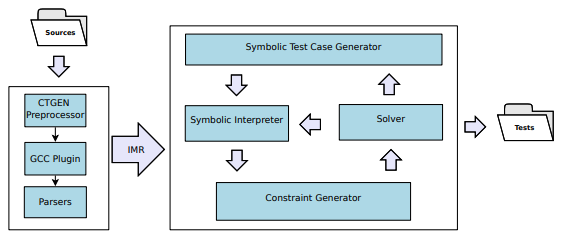
\includegraphics{hinhanh/hinh5}
\end{center}
\caption{Kiến trúc tổng quan của CTGEN}
\end{figure}

\indent Bộ tiền xử lý hoạt động trên mã UUT. Nó bao gồm các chú thích mã tiền xử lý CTGEN, một pluggin GCC biên dịch mã nguồn đã chuẩn bị thành một đặc tả văn bản bao gồm biểu đồ luồng điều khiển (CFG) và thông tin bảng ký hiệu như function signatures, types và variables, trình phân tích cú pháp , chuyển đổi CFG và thông tin bảng ký hiệu thành biễu diễn mô hình trung gian (IMR).

\indent Máy phân tích hoạt động trên IRM, các khối xây dựng của nó và các tương tác của chúng sẽ được mô tả bên dưới. Trình tạo trường hợp kiểm tra tượng trưng (Symbolic Test Case Generator) chịu trách nhiệm cho việc mở rộng các CFG liên quan đến chức năng được kiểm tra và các chức năng phụ của nó. Hơn nữa, nó xử lý việc lựa chọn các đường dẫn, mỗi điểm bắt đầu bằng nút bắt đầu của CFG và chứa các chuyển tiếp chưa được khám phá. Nếu đường dẫn như vậy có thể được tìm thấy, nó được chuyển đến trình thông dịch tượng trưng (Symbolic Interpreter), đi qua đường dẫn và tính toán một cách tượng trưng hiệu quả các câu lệnh của nó trong mô hình bộ nhớ. Ngay khi nút tiếp theo trên đường dẫn được bảo vệ bởi một điều kiện không tầm thường (non-trivial), Trình tạo ràng buộc (Constraint Generator) được gọi và giải quyết tất cả các con trỏ và tham chiếu mảng xảy ra trong điều kiện này. Nó cũng chuyển các ràng buộc kết quả cho bộ giải (Solver). CTGEN sử dụng bộ giải SMT, bộ giải này hỗ trợ các kiểu dữ liệu cơ bản, dấu chấm động, mảng và bit vectors. Nếu bộ giải có thể tìm ra giải pháp cho ràng buộc, giải pháp đó được chuyển lại cho trình thông dịch tượng trưng, tiếp tục đi theo con đường đang xét. Mặt khác, nếu ràng buộc là không khả thi hoặc đường dẫn được hoàn thành bộ giải sẽ chuyển kết quả cho bộ tạo trường hợp thử nghiệm tượng trưng. Nó học được từ tính không khả thi và cố gắng tạo ra một đường dẫn khác chứa các chuyển tiếp vẫn chưa được khám phá hoặc cố gắng tiếp tục đường dẫn đã hoàn thành. Khi không tìm thấy đường dẫn như vậy, unit test được tạo dựa trên các giải pháp được thu thập (nếu có) và được lưu trữ trong hệ thống tệp. 
\subsection{PathCrawler}
PATHCRAWLER là một công cụ tạo bộ thử nghiệm cho các chương trình C. Ban đầu được thiết kế để tự động hóa  kiểm tra đơn vị (Unit test) bằng cách tạo đầu vào thử nghiệm để bao phủ toàn bộ cấu trúc của chương trình C đang thử nghiệm.

\indent PATHCRAWLER đã được phát triển tại CEA List từ năm 2002. Trong những năm qua nó đã được mở rộng để xử lý một tập hợp con lớn hơn của các chương trình C và áp dụng cho nhiều vấn đề phân biệt, thường được áp dụng nhiều nhất trong các phần mềm nhúng. Trong năm 2010, nó đã được cung cấp công khai dưới dạng máy chủ thử nghiệm trực tuyến, để đánh giá và sử dụng trong giảng dạy.

\indent PATHCRAWLER được xây dựng dựa trên kỹ thuật Symbolic execution. Người dùng cung cấp các tệp có thể biên dịch có chứa mã chương trình C hoàn chỉnh của hàm được kiểm tra (gọi là f) và tất cả các hàm khác có thể gọi trực tiếp hoặc gián tiếp bởi hàm f. Họ cũng có thể chọn tiêu chí bảo hiểm và bất kỳ giới hạn nào về số lần lặp lại trong các đường dẫn được bảo hiểm cũng như một điều kiện tiên quyết tùy chọn để xác định bối cảnh thử nghiệm. Công việc tạo bộ thử nghiệm bằng PATHCRAWLER gồm hai giai đoạn chính. Trong giai đoạn đầu tiên, PATHCRAWLER trích xuất các đầu vào của f và tạo ra một khai thác thử nghiệm được sử dụng để thực hiện f trên một trường hợp thử nghiệm nhất định. Khai thác thử nghiệm về cơ bản là một phiên bản cụ thể của mã tạo ra dấu vết của đường dẫn được bao phủ bởi mỗi trường hợp thử nghiệm. Các đầu vào được trích xuất bao gồm các tham số chính thức của f và các biến toàn cục không cố định được sử dụng bởi f. Mỗi trường hợp thử nghiệm sẽ cung cấp một giá trị cho mỗi đầu vào này. Giai đoạn này sử dụng nền tảng FRAMA-C \cite{kirchner2015frama}, được phát triển tại CEA List. Giai đoạn thứ hai tạo ra các đầu vào thử nghiệm để tôn trọng tiêu chí bảo hiểm đã chọn.  Giai đoạn này dựa trên thực thi biểu tượng, tạo ra các ràng buộc đối với các giá trị đầu vào tượng trưng và giải quyết ràng buộc để tìm giải pháp, dưới dạng các giá trị đầu vào cụ thể mới, cho một tập các ràng buộc mới. Thật vậy, thực thi tượng trưng được sử dụng để phân tích dấu vết của đường dẫn thực hiện theo sau khi khai thác thực thi f trên các giá trị đầu vào cụ thể của từng trường hợp thử nghiệm được tạo và tạo ra vị từ đường dẫn xác định các biến đầu vào khiến đường dẫn đó bị che lấp.

\indent Cấu trúc tổng quan của PATCHCRAWLER được minh họa trong Hình 6.
\begin{figure}[ht]
\begin{center}
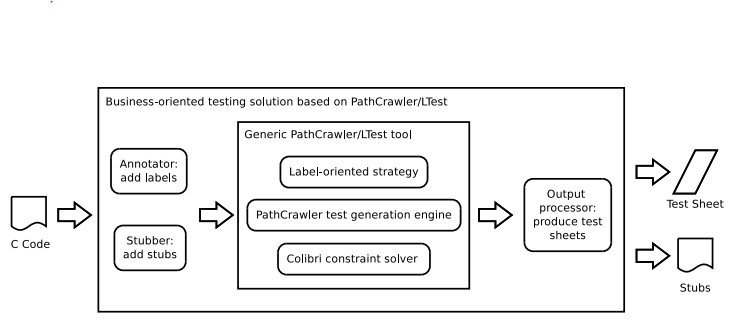
\includegraphics[scale=.7]{hinhanh/pathcrawler}
\end{center}
\caption{Kiến trúc tổng quan của CTGEN}
\end{figure}

Công cụ tạo thử nghiệm chung PATHCRAWLER có ba thành phần chính. Một công cụ kiểm tra đồng thời, PATHCRAWLER, được sử dụng để tạo các trường hợp kiểm thử cho một chương trình C nhất định. Việc tạo các đầu vào kiểm tra cụ thể cho một đường dẫn chương trình nhất định phụ thuộc vào bộ giải ràng buộc, COLIBRI. Cơ chế đặc tả của lable và chiến lược lable-oriented cụ thể cho phép hỗ trợ hiệu quả tiêu chí độ bao phủ thử nghiệm mong muốn được thể hiện dưới dạng lable. Để thích ứng với PATHCRAWLER cho bối cảnh công nghiệp cụ thể, các module bổ sung đã được MERCE, chi nhánh nghiên cứu của đối tác công nghiệp phát triển. Chúng bao gồm ANNOTATOR (thể hiện tiêu chí mục tiêu cụ thể về lable), STUBBER (tạo ra các stubs cần thiết) và PROCESSOR OUTPUT (tạo báo cáo thử nghiệm cần thiết).

\indent PATHCRAWLER khác biệt theo hai cách chính so với các công cụ khác dựa trên sự kết hợp giữa giá trị đầu vào cụ thể và tượng trưng. Giống như các công cụ khác, PATHCRAWLER chạy chương trình đang được thử nghiệm trên từng trường hợp thử nghiệm để khôi phục lại dấu vết của đường dẫn thực thi. Tuy nhiên, trong trường hợp PATHCRAWLER's, thực thi thực tế được chọn thay vì thực thi tượng trưng chỉ vì lý do hiệu quả và để chứng minh rằng thử nghiệm thực sự kích hoạt đường dẫn thực hiện dự định. Không giống các công cụ được thiết kế chủ yếu để tìm lỗi, PATHCRAWLER không sử dụng thực thi thực tế để khôi phục kết quả cụ thể của các phép tính mà nó không thể xử lý. Điều này là do các kết quả này chỉ có thể cung cấp một mô hình chưa hoàn chỉnh của chương trình ngữ nghĩa và chương trình PATHCRAWLER nhằm mục đích bảo hiểm hoàn toàn cho một loại chương trình nhất định thay vì bảo hiểm không đầy đủ cho bất kỳ chương trình nào.

\indent Thật vậy, ngay cả với phạm vi bảo hiểm không đầy đủ, nhiều lỗi thường có thể được phát hiện, nhưng PATHCRAWLER được thiết kế để sử dụng trong các quy trình xác minh chính thức hơn, trong đó phạm vi bảo hiểm phải được định lượng và chứng minh để có thể sử dụng kết hợp với các kỹ thuật phân tích tĩnh \cite{petiot2014test}. Nếu một nhánh hoặc đường dẫn không được bao phủ bởi một thử nghiệm, thì tính không thể đạt được của nhánh hoặc tính không khả thi của đường dẫn phải được thể hiện. Tính đúng đắn và đầy đủ là cần thiết cho sự hài lòng 100\% của một tiêu chí bảo hiểm. Tạo trường hợp thử nghiệm là thăm dò, khi mỗi trường hợp thử nghiệm bao gồm mục tiêu thử nghiệm được tạo và hoàn thành, khi không có trường hợp thử nghiệm đối với một số mục tiêu thử nghiệm có nghĩa là mục tiêu này không khả thi hoặc không thể truy cập được.

\indent Tính đúng đắn của phương pháp PATHCRAWLER được xác minh bằng cách thực hiện cụ thể các trường hợp thử nghiệm được tạo trên phiên bản cụ thể của chương trình đang được thử nghiệm. Dấu vết thu được từ việc thực hiện cụ thể của một trường hợp thử nghiệm xác nhận rằng trường hợp thử nghiệm này thực sự thực thi đường dẫn mà nó được tạo ra.

\indent Tính đầy đủ chỉ có thể được đảm bảo khi tất cả các mục tiêu có thể được bao phủ bởi một số lượng các trường hợp thử nghiệm hợp lý, thực thi tượng trưng thể hiện chính xác ngữ nghĩa của C và giải quyết ràng buộc luôn kết thúc trong một thời gian hợp lý. Lưu ý rằng tính đầy đủ và xác minh tính đúng đắn trên mã công cụ thực sự đòi hỏi phải thực thi biểu tượng các tính năng của chương trình để được điều chỉnh phù hợp với nền tảng đích được thực hiện trong cùng một môi trường. PATHCRAWLER hiện chỉ thích nghi với môi trường phát triển Linux và Intel-based platform. Chiến lược tìm kiếm của phương pháp PATHCRAWLER là đảm bảo lặp lại trên tất cả các đường dẫn khả thi của chương trình, cần thiết cho sự hoàn chỉnh, cho tất cả các chương trình kết thúc với nhiều đường dẫn chính xác. Các chương trình chứa các vòng lặp vô hạn không thể được kiểm tra trong mọi trường hợp theo cách chúng tôi mô tả ở đây, vì việc thực hiện chương trình trên các đầu vào kiểm tra sẽ không bao giờ chấm dứt. Bất kỳ vòng lặp vô hạn nào được đưa vào do lỗi chỉ có thể được phát hiện khi hết thời gian thực hiện từng trường hợp thử nghiệm trên mã được ghi. Việc kết thúc các chương trình có số lượng đường dẫn vô hạn phải có số lượng đầu vào vô hạn và đây là một loại chương trình khác không thể được kiểm tra bằng phương pháp PATHCRAWLER.

\indent Sự khác biệt chính thứ hai giữa PATHCRAWLER và các công cụ tương tự khác là PATHCRAWLER không dựa trên bộ giải số học tuyến tính hoặc bộ giải mã SMT mà dựa trên bộ giải hạn chế miền hữu hạn COLIBRI, cũng được phát triển tại CEA List. Cả PATHCRAWLER và COLIBRI đều được triển khai trong Lập trình logic ràng buộc, tạo điều kiện kiểm soát mức độ phân giải ràng buộc ở mức độ thấp và phát triển các ràng buộc chuyên biệt, cũng như cung cấp cơ chế quay lui hiệu quả.  Trong PATHCRAWLER, các ràng buộc chuyên biệt đã được phát triển để xử lý các hoạt động bit, mảng với bất kỳ số lượng kích thước biến và truy cập mảng nào sử dụng các giá trị chỉ số biến (index value). Nỗ lực điều trị chính xác tất cả các hướng dẫn C đang diễn ra nhưng PATHCRAWLER có thể đã xử lý một lớp lớn các chương trình C.

\indent PathCrawler đưa ra kết quả chi tiết dưới dạng các tệp XML. Chúng bao gồm số liệu thống kê tổng thể về phiên kiểm tra, bao gồm các kết quả về phạm vi bao phủ, cho dù phiên kết thúc bình thường hay hết giờ hoặc bị lỗi và thời gian bắt đầu và kết thúc. Đối với mỗi trường hợp thử nghiệm, các giá trị đầu vào, kết quả, đường dẫn được bao phủ và giá trị đầu ra cụ thể được cung cấp. Kết quả là sự phán quyết theo xác nhận của người dùng nếu được cung cấp hoặc có thể là lỗi thời gian chạy, hết thời gian hoặc phát hiện biến đơn vị. Các giá trị đầu ra tượng trưng cũng được đưa ra. Ngoài ra, đối với mỗi tiền tố đường dẫn không thể được bao phủ, lý do được đưa ra: thể hiện tính không khả thi, thời gian chờ giải quyết ràng buộc, giới hạn số lần lặp lại hoặc xây dựng ngôn ngữ C chưa được xử lý. Vị từ (the predicate) trên các biến đầu vào của từng đường dẫn được bao phủ và tiền tố không được che chở cũng được đưa ra. Trong trường hợp tiền tố đường dẫn được tìm thấy là không khả thi, vị từ có thể được sử dụng để giải thích tính không khả thi cho người dùng và trong trường hợp hết thời gian giải quyết ràng buộc, nó có thể được sử dụng để xác định tính khả thi của đường dẫn theo cách thủ công.
\subsection{Klee}
Klee là một công cụ có khả năng tự động tạo ra các thử nghiệm đạt được độ bao phủ cao trên một loạt các chương trình phức tạp và chuyên sâu về môi trường. Công cụ này sử dụng kỹ thuật Symbolic execution. Các thử nghiệm do KLEE tạo ra đạt được độ bao phủ cao, trung bình trên 90\% cho mỗi công cụ và đánh bại đáng kể mức độ bao phủ của các bộ thử nghiệm viết tay của nhà phát triển.

\indent KLEE được thiết kế để kiểm tra sâu, mạnh mẽ một loạt các ứng dụng, tận dụng các thành phần từ công cụ có trước là EXE \cite{cadar2008exe}. KLEE sử dụng một loạt các tối ưu hóa giải quyết ràng buộc, thể hiện các trạng thái chương trình một cách gọn gàng và sử dụng các phương pháp tìm kiếm để có được phạm vi bao phủ mã cao. Ngoài ra, nó sử dụng một cách tiếp cận đơn giản và dễ hiểu để đối phó với môi trường bên ngoài. Các tính năng này cải thiện hiệu suất của KLEE kèm theo một mức độ lớn và cho phép nó kiểm tra một loạt các chương trình chuyên sâu về hệ thống “out of the box”.

\indent Các bài kiểm tra được tạo tự động của KLEE, có độ bao phủ cao trên một loạt các chương trình thực tế, phức tạp và chuyên sâu về môi trường. Đánh giá chuyên sâu nhất của chúng tôi áp dụng KLEE cho tất cả 89 chương trình 1 trong phiên bản ổn định mới nhất của GNU COREUTILS (phiên bản 6.10), chứa khoảng 80.000 dòng mã thư viện và 61.000 dòng trong các tiện ích thực tế. Các chương trình này tương tác rộng rãi với môi trường của chúng để cung cấp nhiều chức năng, bao gồm quản lý hệ thống tệp (ví dụ: ls, dd, chmod), hiển thị và định cấu hình các thuộc tính hệ thống (ví dụ: logname, printenv, hostname), kiểm soát lệnh gọi (ví dụ: nohup, nice, env), xử lý tệp văn bản (ví dụ: sort, od, patch), v.v. Chúng tạo thành môi trường cấp độ người dùng cốt lõi được cài đặt trên nhiều hệ thống Unix. Chúng được sử dụng hàng ngày bởi hàng triệu người, sửa lỗi được xử lý kịp thời và các bản phát hành mới được đẩy thường xuyên. Hơn nữa, tìm lỗi trong COREUTILS là khó. Chúng được cho là bộ ứng dụng nguồn mở được thử nghiệm tốt nhất hiện có. Năm 1995, thử nghiệm ngẫu nhiên một tập hợp con các tiện ích COREUTILS đã tìm thấy ít lỗi hơn so với bảy hệ thống Unix thương mại \cite{miller2000re}. Lỗ hổng COREUTILS cuối cùng được báo cáo trên cơ sở dữ liệu SecurityFocus hoặc US National Vulnerability là ba năm trước.

\indent KLEE tìm thấy các lỗi quan trọng trong mã được kiểm tra nhiều. Nó đã tìm thấy mười lỗi nghiêm trọng trong COREUTILS (bao gồm ba lỗi đã thoát khỏi sự phát hiện trong 15 năm), trong đó có nhiều lỗi xảy ra hơn so với báo cáo năm 2006, 2007 và 2008. Thực tế là các trường hợp kiểm tra KLEE có thể được chạy trên phiên bản thô của mã (ví dụ: được biên dịch bằng gcc) giúp đơn giản hóa rất nhiều việc gỡ lỗi và báo cáo lỗi.

\indent KLEE có hai mục tiêu: (1) đạt mọi dòng mã thực thi trong chương trình và (2) phát hiện tại mỗi hoạt động nguy hiểm (ví dụ: quy định, xác nhận) nếu có bất kỳ giá trị đầu vào nào tồn tại có thể gây ra lỗi. KLEE làm như vậy bằng cách chạy các chương trình một cách tượng trưng: không giống như thực thi thông thường, nơi các hoạt động tạo ra các giá trị cụ thể từ toán hạng của chúng, ở đây chúng tạo ra các ràng buộc mô tả chính xác tập hợp các giá trị có thể trên một đường dẫn cụ thể. Khi KLEE phát hiện ra lỗi hoặc khi một đường dẫn đến một lệnh gọi thoát, KLEE sẽ giải quyết các ràng buộc của đường dẫn hiện tại (được gọi là kết nối đường dẫn của nó) để tạo ra một trường hợp thử nghiệm sẽ đi theo cùng một đường dẫn khi chạy lại trên một phiên bản chưa được sửa đổi của kiểm tra chương trình (ví dụ, được biên dịch với gcc).

\indent KLEE được thiết kế sao cho các đường dẫn được theo sau bởi chương trình chưa sửa đổi sẽ luôn đi theo cùng một đường dẫn mà KLEE đã thực hiện (tức là không có kết quả tích cực giả). Tuy nhiên, tính không xác định trong mã được kiểm tra và lỗi trong KLEE hoặc các mô hình của nó đã tạo ra kết quả tích cực giả trong thực tế. Khả năng chạy lại các bài kiểm tra bên ngoài KLEE, kết hợp với các công cụ tiêu chuẩn như gdb và gcov là vô giá để chẩn đoán các lỗi đó và để xác nhận kết quả của chúng tôi.

\indent Tiếp theo tôi sẽ trình cái nhìn tổng quan về cách thức hoạt động của nó.

\indent KLEE là một thiết kế lại hoàn chỉnh của hệ thống đã có trước đây EXE. Ở mức cao, KLEE hoạt động như một sự kết hợp giữa một hệ điều hành cho các quy trình tượng trưng và trình thông dịch. Mỗi quá trình biểu tượng có một tệp đăng ký, ngăn xếp, bộ đếm chương trình và điều kiện đường dẫn. Để tránh nhầm lẫn với quy trình Unix, chúng tôi đề cập đến đại diện KLEE của một quy trình tượng trưng như một trạng thái. Các chương trình được biên dịch sang ngôn ngữ hợp ngữ LLVM \cite{lattner2004llvm}, một tập lệnh ảo giống như RISC. KLEE trực tiếp diễn giải tập lệnh này và ánh xạ các hướng dẫn đến các ràng buộc mà không cần xấp xỉ.

\indent Bất cứ lúc nào, KLEE có thể đang thực thi một số lượng lớn các trạng thái. Cốt lõi của KLEE là một vòng lặp thông dịch chọn một trạng thái để chạy và sau đó thực hiện một cách tượng trưng một lệnh trong ngữ cảnh của trạng thái đó. Vòng lặp này tiếp tục cho đến khi không còn trạng thái nào nữa hoặc đạt đến thời gian chờ do người dùng xác định.

\indent Không giống như một quy trình thông thường, các vị trí lưu trữ cho một thanh ghi trạng thái, các đối tượng stack và heap sẽ tham chiếu các biểu thức  thay vì các giá trị dữ liệu thô. Các thành phần của biểu thức là các biến hoặc hằng biểu tượng và các nút bên trong đến từ các hoạt động ngôn ngữ assembly LLVM (ví dụ: các phép toán số học, thao tác bitwise, so sánh và truy cập bộ nhớ). Các vị trí lưu trữ giữ một biểu thức không đổi được gọi là cụ thể.

\indent Thực hiện tượng trưng của phần lớn các hướng dẫn là đơn giản. Ví dụ, để thực hiện một cách tượng trưng một lệnh LLVM add:

\begin{center}
\%dst = add i32 \%src0, \%src1
\end{center}

\indent KLEE truy xuất các phần bổ sung từ các thanh ghi \%src0 và \%src1 và viết một biểu thức mới add (\%src0, \%src1) vào thanh ghi \%dst. Để có hiệu quả, mã xây dựng biểu thức sẽ kiểm tra xem tất cả các toán hạng đã cho có cụ thể không (ví dụ: hằng số) và, nếu vậy, thực hiện thao tác chính, trả về một biểu thức không đổi.

\indent Các nhánh có điều kiện lấy một biểu thức boolean (điều kiện nhánh) và thay đổi con trỏ lệnh của trạng thái dựa trên điều kiện là đúng hay sai. KLEE truy vấn bộ giải ràng buộc để xác định xem điều kiện nhánh là có thể đúng hoặc có thể chứng minh sai dọc theo đường dẫn hiện tại; nếu vậy, con trỏ lệnh được cập nhật đến vị trí thích hợp. Mặt khác, cả hai nhánh đều có thể: KLEE nhân bản trạng thái để nó có thể khám phá cả hai đường dẫn, cập nhật con trỏ lệnh và điều kiện đường dẫn trên mỗi đường dẫn một cách thích hợp.

\indent Các hoạt động nguy hiểm tiềm tàng tạo ra các nhánh kiểm tra xem có tồn tại bất kỳ giá trị đầu vào nào có thể gây ra lỗi không. Ví dụ, một lệnh chia tạo ra một nhánh kiểm tra ước số bằng không. Các nhánh như vậy làm việc giống hệt với các nhánh bình thường. Do đó, ngay cả khi kiểm tra thành công (nghĩa là đã phát hiện lỗi), việc thực thi vẫn tiếp tục trên đường dẫn sai, điều này thêm vào phủ định của kiểm tra dưới dạng một ràng buộc (ví dụ: làm cho ước số không bằng 0). Nếu phát hiện lỗi, KLEE tạo trường hợp kiểm tra để kích hoạt lỗi và chấm dứt trạng thái.

\indent Cũng như các hoạt động nguy hiểm khác, tải và lưu trữ các cấu trúc tạo ra các kiểm tra: trong trường hợp này để kiểm tra xem địa chỉ nằm trong giới hạn của một đối tượng bộ nhớ hợp lệ. Tuy nhiên, hoạt động tải và lưu trữ trình bày một biến chứng bổ sung. Đại diện đơn giản nhất của bộ nhớ được sử dụng bởi mã được kiểm tra sẽ là một mảng byte. Trong trường hợp này, tải và lưu trữ sẽ chỉ đơn giản là ánh xạ tới các biểu thức đọc và ghi tương ứng. Thật không may, STP bộ giải ràng buộc của chúng tôi gần như không thể giải quyết được các ràng buộc kết quả (và cả các bộ giải hạn chế khác mà chúng tôi biết). Do đó như trong EXE, KLEE ánh xạ mọi đối tượng bộ nhớ trong mã được kiểm tra thành một mảng STP riêng biệt (theo nghĩa nào đó, ánh xạ một không gian địa chỉ phẳng thành một phân đoạn). Biểu diễn này cải thiện đáng kể hiệu năng vì nó cho phép STP bỏ qua tất cả các mảng không được tham chiếu bởi một biểu thức đã cho. 

\indent Nhiều hoạt động (chẳng hạn như kiểm tra ràng buộc hoặc sao chép mức ghi đối tượng) yêu cầu thông tin cụ thể của đối tượng. Nếu một con trỏ có thể tham chiếu đến nhiều đối tượng, các thao tác này trở nên khó thực hiện. Để đơn giản, KLEE vượt qua vấn đề này như sau. Khi một con trỏ được ước tính p có thể tham chiếu đến N đối tượng, KLEE nhân bản trạng thái hiện tại N lần. Trong mỗi trạng thái, nó ràng buộc p nằm trong giới hạn của đối tượng tương ứng và sau đó thực hiện thao tác đọc hoặc ghi thích hợp. Mặc dù phương pháp này có thể tốn kém cho các con trỏ có bộ điểm lớn, nhưng hầu hết các chương trình chúng tôi đã thử nghiệm chỉ sử dụng các con trỏ tượng trưng liên quan đến một đối tượng và KLEE được tối ưu hóa tốt cho trường hợp này.

\section{Tổng quan về công cụ đánh giá tự động}

\subsection{Đặt vấn đề}

Mục tiêu công việc của tôi là tự động quyết định tính chính xác của các bài tập lập trình của sinh viên theo một giải pháp (solution) cho trước. Để cụ thể hơn, giáo viên sẽ đưa ra một đề bài tập và một giải pháp (solution) tương ứng với đề bài chính xác nhất cho bài tập lập trình và sinh viên sau khi hoàn thành bài tập sẽ nộp lại bài làm của mình. Mục tiêu của tôi là quyết định bài tập của sinh viên và solution của giáo viên có hành xử giống nhau hay không. Để giải quyết mục tiêu đó tôi tìm cách cung cấp câu trả lời có hoặc không cho câu hỏi sau: bài làm của sinh viên có cho ra output giống như là output của solution hay không.

Giả sử một bài tập lập trình yêu cầu học sinh viết hàm max trả về giá trị lớn nhất của 3 tham số đầu vào số nguyên. Giáo viên sẽ cung cấp solution như (hình a) và chúng tôi nhận được các bài giải của sinh viên (hình b và c) trong đó bài nộp của sinh viên trong hình b là đúng và bài nộp trong hình c là không đúng. Đối với bài nộp đúng sẽ cho ra output giống với output của solution, và các bài nộp không đúng vì bỏ qua các điều kiện biên sẽ cho ra output không giống với output của solution. Cho bộ input đầu vào 
a=5, b=5, c=3 thì đoạn code solution và đoạn code của sinh viên 1 sẽ cho ra kết quả là 5 còn đoạn code của sinh viên thứ 2 cho ra kết quả là 3 và rõ ràng đoạn code của sinh viên thứ 2 đã cho kết quả không đúng như mọng đợi.Và trong bài viết này tôi hy vọng công cụ chấm điểm của tôi sẽ cho ra kết quả đúng dựa trên các bộ testcase có sẵn.

\begin{lstlisting}[language=c]
int max(int a, int b, int c) 
{
    if(a >= b && a>= c){
        return a;
    } else if(b >=a && b>=c){
        return b;
    } else{
        return c;
    }
}
\end{lstlisting}
\caption{Hình a. Solution}

\begin{lstlisting}[language=c]
int max(int a, int b, int c) 
{ 
    if (a>=b){
        if (a>=c){
            return a;
        }
        else{
            return c;
    else{
        if (b>=c){
            return b;
        }
        else{
            return c; 
        }
    }
}
\end{lstlisting}
\caption{Hình b. Sinh viên 1}

\begin{lstlisting}[language=c]
int max(int a, int b, int c) 
{ 
    if (a>b && a>c){
        return a;
    } else if(b>a && b>c){
        return b;
    } else{
        return c;
    }
}
\end{lstlisting}
\caption{Hình c. Sinh viên 1}

\subsection{Ý tưởng chính}
Trước khi đi vào ý tưởng chính để tạo ra một công cụ chấm điểm tự động thì tôi muốn nói đến khái niệm về công cụ chấm điểm tự động.

Công cụ chấm điểm tự động là một bộ chương trình giúp bạn tự động sinh ra các bộ input testcase mẫu hoặc sử dụng các bộ testcase đã được tạo sẵn và sau đó chạy 2 chương trình lời giải khác nhau với các bộ testcase mẫu để so sánh output với nhau. Ở đây lời giải 1 chính là file solution của giáo viên đưa ra còn lời giải 2 chính là bài nộp của sinh viên sau khi làm bài.

Sử dụng công cụ chấm điểm tự động là một trong những cách chấm điểm bài thi hiệu quả nhất. Với cách chấm điểm thủ công việc sai sót nhỏ (bỏ qua các giá trị biên) là rất khó tránh khỏi và công cụ chấm điểm tự động được làm ra để giải quyết vấn đề đó. Công cụ chấm điểm tự động yêu cầu một bài giải mẫu được cho trước và một bài tập của sinh viên và so sánh kết quả của hai chương trình này với nhau. Nếu công cụ chấm điểm tự động phát hiện được có một bộ testcase mà kết quả của hai chương trình cho ra khác nhau thì bài tập của sinh viên đưa vào là không đúng. Còn nếu tất các các bộ testcase đều đúng thì bài tập của sinh viên nộp bài là đúng.

Một công cụ chấm điểm tự động bao gồm các thành phần chính như sau:
\begin{itemize}
\item[-] \textbf{Lời giải của solution}
\item[-] \textbf{Lời giải của sinh viên}
\item[-] \textbf{Nơi chưa các bộ testcase}
\item[-] \textbf{Trình so test}
\end{itemize}

Lời giải của soluotion thông thường sẽ được giáo viên thực hiện trong khi ra đề. Lời giải này thông thường sẽ là lời giải đúng nhất và chạy đúng hết các bộ testcase đưa ra. Công cụ chấm điểm tự động sẽ cho ra kết quả bài tập của sinh viên dựa trên kết quả của solution này.

Lời giải của sinh viên là bài nộp của sinh viên sau khi kết thúc phần thi.

Nơi chứa các bộ testcase là một file bao gồm hai thông tin đó là: số bộ testcase và các bộ testcase tương ứng. Các bộ testcase sẽ được sinh ra tự động theo hai cách đó là: sử dụng tool sinh testcase tự động đối với các trường hợp input đầu vào là các kiểu dự liệu nguyên thủy như int, float,... còn đối với input đầu vào có kiểu phức tạp hơn như Array thì tôi sẽ viết một hàm sinh test case tự động. Hàm sinh test case tự động này sẽ chạy đầu tiên trong công cụ chấm điểm để đảm bảo cung cấp các bộ testcase một cách đầy đủ.

Trình so test là thành phần quan trọng giúp đưa ra điểm số cuối cùng cho bài tập của sinh viên. Để có thể đưa ra được kết quả thì trình so test phải thực thi lần lượt lời giải của solution và lời giải của sinh viên với input đầu vào là bộ testcase được sinh sẵn, sau khi thực thi xong sẽ cho ra hai file chứa output của solution và sinh viên. Kết quả chỉ đúng khi output của solution và sinh viên là giống nhau. Và việc thực thi này được lặp lại n lần với n là số bộ testcase được lưu trong file chưa testcase. Sau khi thực thi xong n lần thì trình so test sẽ có được số lần thực thi đúng và số lần thực thi không đúng và dựa vào kết quả đó để cho ra điểm số cuối cùng.

\subsection{Cách sinh testcase tự động}

Để xây dụng được một công cụ chấm điểm tự động với độ chính xác cao đòi hỏi bạn phải có được các bộ testcase chính xác, có độ bao phủ cao. Các bộ testcase phải duyệt qua hết các nhánh của chương trình để đảm bảo không bỏ xót các trường hợp đặc biệt hoặc bị xót khi kiểm tra đối với các giá trị biên.

Việc xây dựng thủ công các bộ testcase thử nghiệm đòi hỏi rất nhiều thời gian và công sức. Và đối với việc xây dựng các bộ testcase một cách thủ công rất dễ đem lại nhiều thiếu xót dẫn đến kết quả chấm điểm của công cụ không được chính xác. Vì vậy trong bài này tôi sử dụng công cụ sinh testcase tự đông Klee để xây dựng các bộ testcase cho bài tập lập trình của sinh viên.

Klee là công cụ tự sinh testcase tự động mã nguồn mở, được xây dựng trên cơ sở hạ tầng trình biên dịch LLVM. Klee sử dụng kỹ thuật Symbolic execution và có khả năng tự tạo ra các bộ testcase đạt được độ bao phủ cao trên một loạt các chương trình phức tạp và chuyên sâu về môi trường.

Có 2 cách cài đặt Klee:
\begin{itemize}
\item[-] \textbf{Cài đặt Klee bằng Docker}
\item[-] \textbf{Cài đặt Klee bằng LLVM 6.0}
\end{itemize}

\subsubsection{Cài đặt Klee bằng Docker}
Trước khi đi vào cài đặt chúng ta cần tìm hiểu để biết Docker là gì.

Docker là một nền tảng cho developers và system admin để develop, deploy và run application với container. Nó cho phép tạo các môi trường độc lập và tách biệt để khởi chạy và phát triển ứng dụng và môi trường này được gọi là container. Khi cần deploy lên bất kỳ server nào chỉ cần run container của Docker thì application của bạn sẽ được khởi chạy ngay lập tức.

Docker cung cấp các công cụ để triển khai các ứng dụng trong các container. Các container được (phần lớn) cách ly với nhau, điều này cho phép bạn tạo một KLEE container, sửa lại và sau đó bỏ nó đi khi bạn thực hiện mà không ảnh hưởng đến hệ thống cơ bản hoặc các thùng chứa khác.

Một Docker container được xây dựng từ một Docker image. Docker image gói gọn một ứng dụng trong trường hợp này là KLEE. Việc đóng gói ở cấp độ ứng dụng này rất hữu ích vì nó cung cấp một môi trường có thể tái tạo và có thể tái tạo được để chạy KLEE.

Có 2 cách để có được Klee Docker image:

\textbf{Pulling from the Docker Hub}

Để tải về một Klee Docker image phiên bản mới nhất chúng ra thực hiện lệnh như sau:

\begin{figure}[ht]
\begin{center}
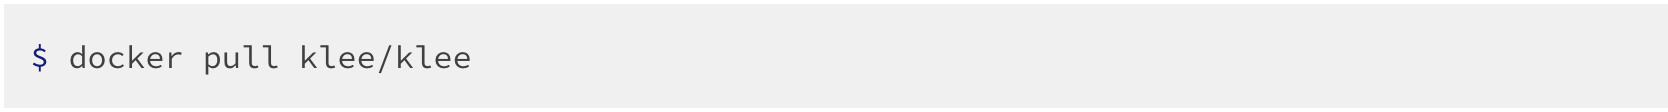
\includegraphics[scale=.3]{hinhanh/pulldocker.png}
\end{center}
\end{figure}

Nếu bạn muốn sử dụng một phiên bản cụ thể của Klee bạn nên thực hiện lệnh như sau:

\begin{figure}[ht]
\begin{center}
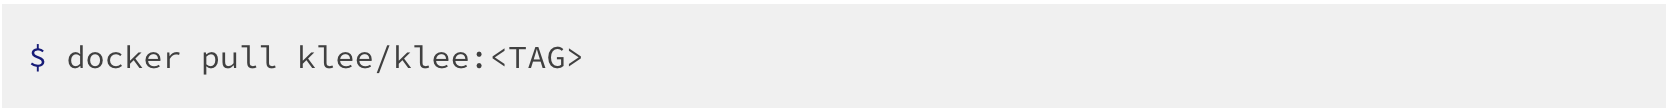
\includegraphics[scale=.3]{hinhanh/pulldockertag.png}
\end{center}
\end{figure}

\textbf{Building the Docker image locally}

Nếu bạn muốn tải một Klee Docker image một cách thủ công thay vì tải về từ Docker hub, bạn có thể làm như vậy bằng cách thực hiên các lệnh sau:

\begin{figure}[ht]
\begin{center}
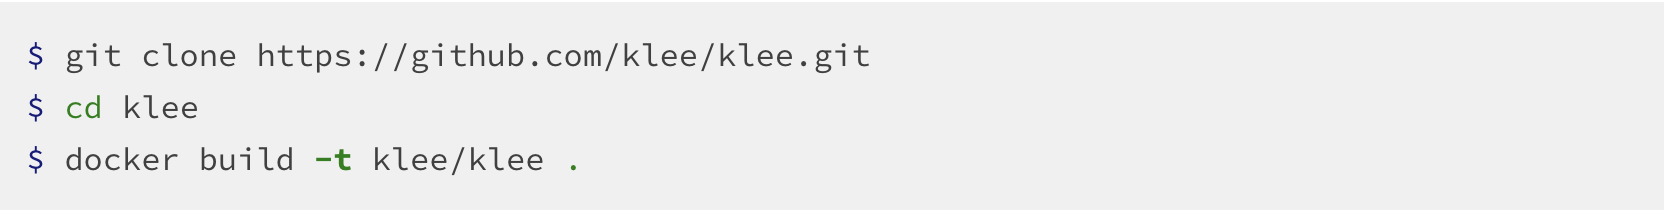
\includegraphics[scale=.3]{hinhanh/builddockerlocal.png}
\end{center}
\end{figure}

Hệ thống sẽ sử dụng nội dung của Dockerfile trong thư muc klee để xây dựng Klee Docker image.

Sau khi tải về máy Klee Docker image, chúng ta sẽ tiếp tục tạo một Klee Docker container để có thể  sử dụng được công cụ klee. Cách đơn giản để tạo được một Klee Docker container và có được quyền truy cập shell, bạn cần thực hiện lệnh như sau:

\begin{figure}[ht]
\begin{center}
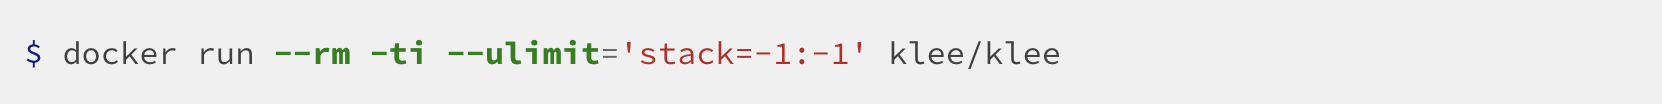
\includegraphics[scale=.3]{hinhanh/kleecontainer.png}
\end{center}
\end{figure}

Nếu bạn muộn tạo một container của Klee với phiên bản cụ thể bạn chỉ cần thay thế klee/klee bằng klee/klee:<tag> trong đó <tag> là phiên bản Klee bạn muốn tạo.

Tùy chọn --ulimit đặt kích thước ngăn xếp không giới hạn bên trong container. Điều này là để tránh các sự cố tràn ngăn xếp khi chạy KLEE.

Tùy chọn --rm được sử dụng với lệnh Docker dùng để hủy container khi ứng dụng chạy trong container (/bin /bash) bị chấm dứt. 

Nếu câu lệnh trên thực hiện chính xác, dấu nhắc shell của bạn sẽ thay đổi và bạn trở thành người sử dụng klee. (như hình bên dưới)

\begin{figure}[ht]
\begin{center}
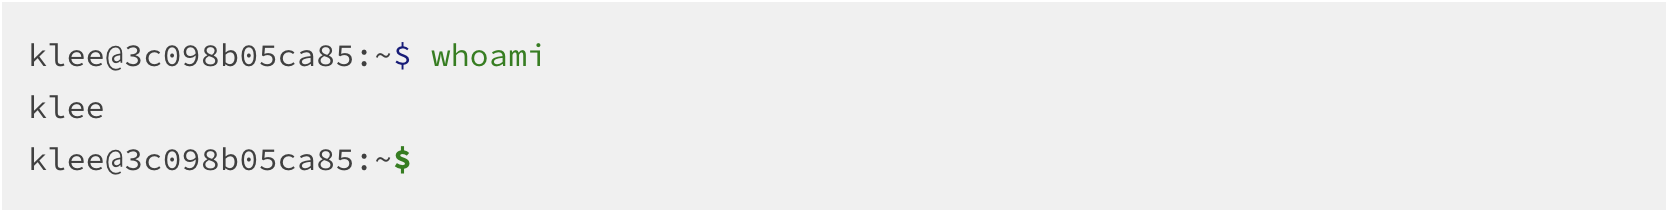
\includegraphics[scale=.3]{hinhanh/shellcontainerklee.png}
\end{center}
\end{figure}

Bây giờ bạn có thể thử chạy klee bên trong container với một số câu lệnh  như kiểm tra phiên bản Klee như hình bên dưới.

\begin{figure}[ht]
\begin{center}
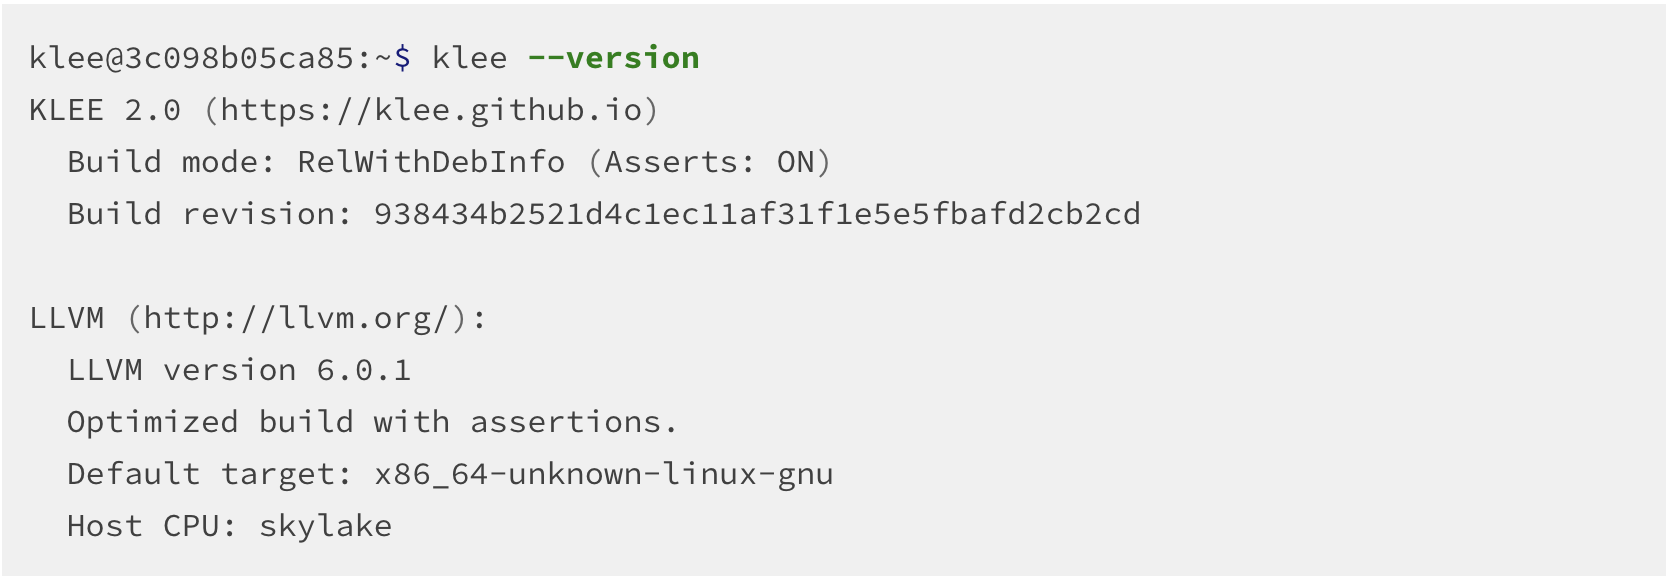
\includegraphics[scale=.3]{hinhanh/kleeversion.png}
\end{center}
\end{figure}

Hoặc là kiểm tra phiên bản clang với câu lệnh như sau: 

\begin{figure}[ht]
\begin{center}
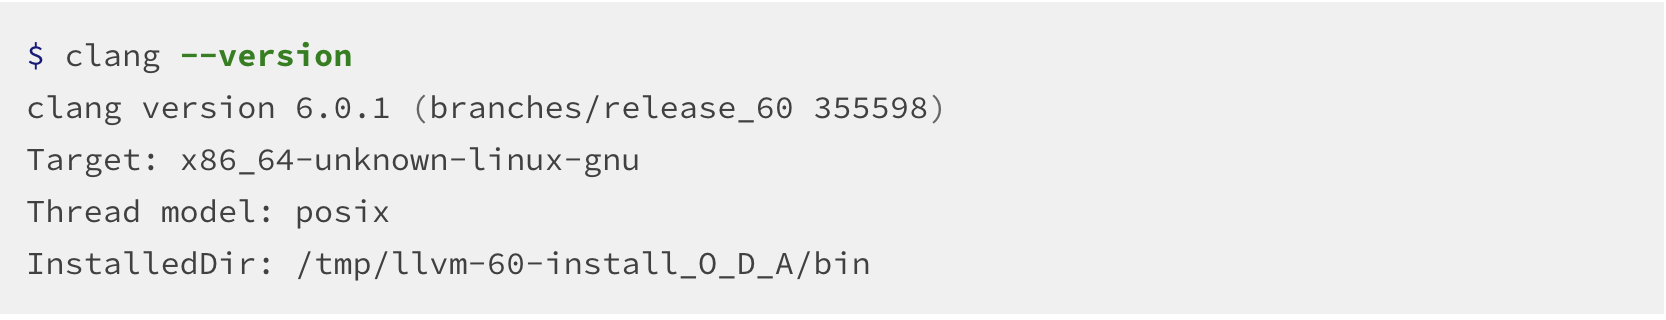
\includegraphics[scale=.3]{hinhanh/clangversion.png}
\end{center}
\end{figure}

Thực thi câu lệnh exit đê thoát khỏi container.

\begin{figure}[ht]
\begin{center}
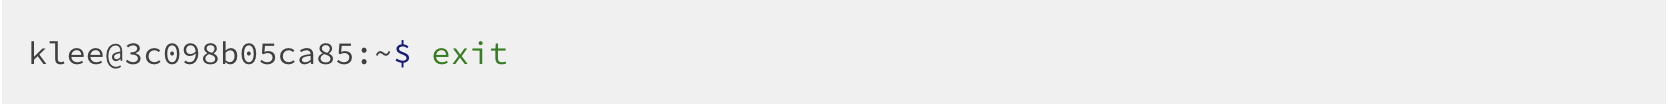
\includegraphics[scale=.3]{hinhanh/exitcontainer.png}
\end{center}
\end{figure}

\subsubsection{Cài đặt Klee bằng LLVM 6.0}

Trước khi đi vào cài đặt thì chúng ta tìm cùng tìm hiểu xem LLVM là gì và nó dùng để làm gì.

LLVM là một tập hợp các công nghệ trình biên dịch và chuỗi công cụ, có thể được sử dụng để phát triển front-end cho bất kỳ ngôn ngữ lập trình nào và back-end cho bất kỳ kiến trúc tập lệnh nào. LLVM được thiết kế xung quanh một đại diện trung gian độc lập với ngôn ngữ (IR), hoạt động như một ngôn ngữ lắp ráp cấp cao, di động, có thể được tối ưu hóa với nhiều biến đổi qua nhiều lần chuyển đổi.

LLVM được viết bằng C ++ và được thiết kế để tối ưu hóa thời gian biên dịch, thời gian liên kết và thời gian chạy. Được triển khai lần đầu cho C và C++, thiết kế không phân biệt ngôn ngữ của LLVM đã tạo ra một loạt các front-end cho rất nhiều ngôn ngữ lập trình. các ngôn ngữ có trình biên dịch sử dụng LLVM bao gồm C\#, Common Lisp, Crystal, CUDA, D, Delphi, Dylan, Fortran, Graphical G Programming Language, Halide, Haskell, Julia, Kotlin, Lua, Objective-C, Ruby, Rust, Scala, Swift.

Một số chức năng của LLVM:

LLVM có thể cung cấp các lớp giữa của một hệ thống trình biên dịch hoàn chỉnh, lấy mã đại diện trung gian (IR: Intermediate Representation) từ trình biên dịch và phát ra một IR được tối ưu hóa. IR mới này sau đó có thể được chuyển đổi và liên kết thành mã ngôn ngữ lắp ráp phụ thuộc vào máy cho một nền tảng đích. LLVM có thể chấp nhận IR từ chuỗi công cụ GNU Compiler Collection (GCC), cho phép nó được sử dụng với một loạt các trình biên dịch mở rộng được viết cho dự án đó.

LLVM cũng có thể tạo mã máy có thể định vị lại tại thời gian biên dịch hoặc thời gian liên kết hoặc thậm chí mã máy nhị phân tại thời gian chạy.

LLVM hỗ trợ một tập lệnh và hệ thống loại độc lập với ngôn ngữ. Mỗi lệnh ở dạng gán đơn tĩnh (SSA: Static Single Assignment), nghĩa là mỗi biến (được gọi là thanh ghi) được gán một lần và sau đó được đóng băng. Điều này giúp đơn giản hóa việc phân tích các phụ thuộc giữa các biến. LLVM cho phép mã được biên dịch tĩnh, vì nó nằm trong hệ thống GCC truyền thống hoặc còn lại để biên dịch muộn từ IR sang mã máy thông qua quá trình biên dịch đúng lúc (JIT: Just-in-time), tương tự như Java. Hệ thống loại bao gồm các loại cơ bản như số nguyên hoặc số dấu phẩy động và năm loại dẫn xuất: con trỏ, mảng, vectơ, cấu trúc và hàm. Một cấu trúc kiểu trong một ngôn ngữ cụ thể có thể được biểu diễn bằng cách kết hợp các loại cơ bản này trong LLVM. Ví dụ, một lớp trong C++ có thể được biểu diễn bằng hỗn hợp các cấu trúc, hàm và mảng của các con trỏ hàm.

Trình biên dịch LLVM JIT có thể tối ưu hóa các nhánh tĩnh không cần thiết ra khỏi chương trình khi chạy và do đó rất hữu ích để đánh giá một phần trong trường hợp chương trình có nhiều tùy chọn, hầu hết có thể dễ dàng được xác định là không cần thiết trong một môi trường cụ thể. Tính năng này được sử dụng trong đường ống OpenGL của Mac OS X Leopard (v10.5) để cung cấp hỗ trợ cho các tính năng phần cứng bị thiếu.

Tiếp theo chúng ta đi vào các bước cài đặt công cụ Klee bằng LLVM:

Cài đặt các dependencies: KLEE yêu cầu tất cả các phụ thuộc của LLVM. Đặc biệt, bạn nên cài đặt các chương trình và thư viện được liệt kê bên dưới.

Đối với ubuntu, thực hiện các lệnh sau:

\$ sudo apt-get install build-essential curl libcap-dev git cmake libncurses5-dev python-minimal python-pip unzip libtcmalloc-minimal4 libgoogle-perftools-dev libsqlite3-dev doxygen

\$ pip3 install tabulate

Đối với MacOS, thực hiện các lệnh sau:

\$ brew install curl git cmake python unzip gperftools sqlite3 doxygen bash

\$ pip3 install tabulate

Nếu bạn gặp vấn đề với 'the compiler not finding standard headers under macOS', hãy thử chạy lệnh sau:

\$ open /Library/Developer/CommandLineTools/Packages/macOS\_SDK\_headers\_for\_macOS\_10.14.pkg

Tiếp theo chúng ta sẽ tiến hành cài đặt LLVM 6.0. Nếu bạn đang sử dụng Ubuntu hay Debian thì thực hiện câu lệnh sau:

\$ sudo apt-get install clang-6.0 llvm-6.0 llvm-6.0-dev llvm-6.0-tools

Đối với MacOS, thực hiện câu lệnh sau:

\$ brew install llvm@6

Tiếp theo chúng ta cài đặt bộ constraint solver:

KLEE hỗ trợ nhiều bộ constraint solver khác nhau như STP, Z3, metaSMT,... . Bạn phải cài đặt ít nhất một cái để xây dựng KLEE.

Tiếp theo chúng ta cần tạo một folder mới để chứa mã nguồn (code) của Klee. Để có được mã nguồn của Klee chúng ta thực hiện câu lệnh sau:

\$ git clone https://github.com/klee/klee.git

Sau khi tải mã nguồn Klee từ git về chúng ta tiến hành cấu hình Klee.

KLEE phải được xây dựng “out of source”, vì vậy trước tiên hãy tạo một thư mục build. Bạn có thể tạo cái này bất cứ nơi nào bạn thích. Dưới đây, tôi giả sử bạn tạo thư mục này trong kho lưu trữ KLEE.

\$ mkdir build

Bây giờ bạn truy cập vào thư mục build vừa tạo bằng câu lệnh cd và chạy CMake để định cấu hình KLEE trong đó với <KLEE\_SRC\_DIRECTORY> là đường dẫn đến kho lưu trữ git KLEE mà bạn đã tải về trong bước trên. <CMAKE\_OPTIONS> là các tùy chọn cấu hình. Để biết thêm các tùy chọn cấu hình bạn vào xem trong file README-CMake.md trong kho lưu trữ git Klee.

\$ cd build

\$ cmake <CMAKE\_OPTIONS> <KLEE\_SRC\_DIRECTORY>

Ví dụ: nếu bạn muốn xây dựng KLEE với STP, thời gian chạy POSIX, klee-uclibc và kiểm tra đơn vị (Unit testing) thì dòng lệnh sẽ trông giống như thế này.

\begin{figure}[ht]
\begin{center}
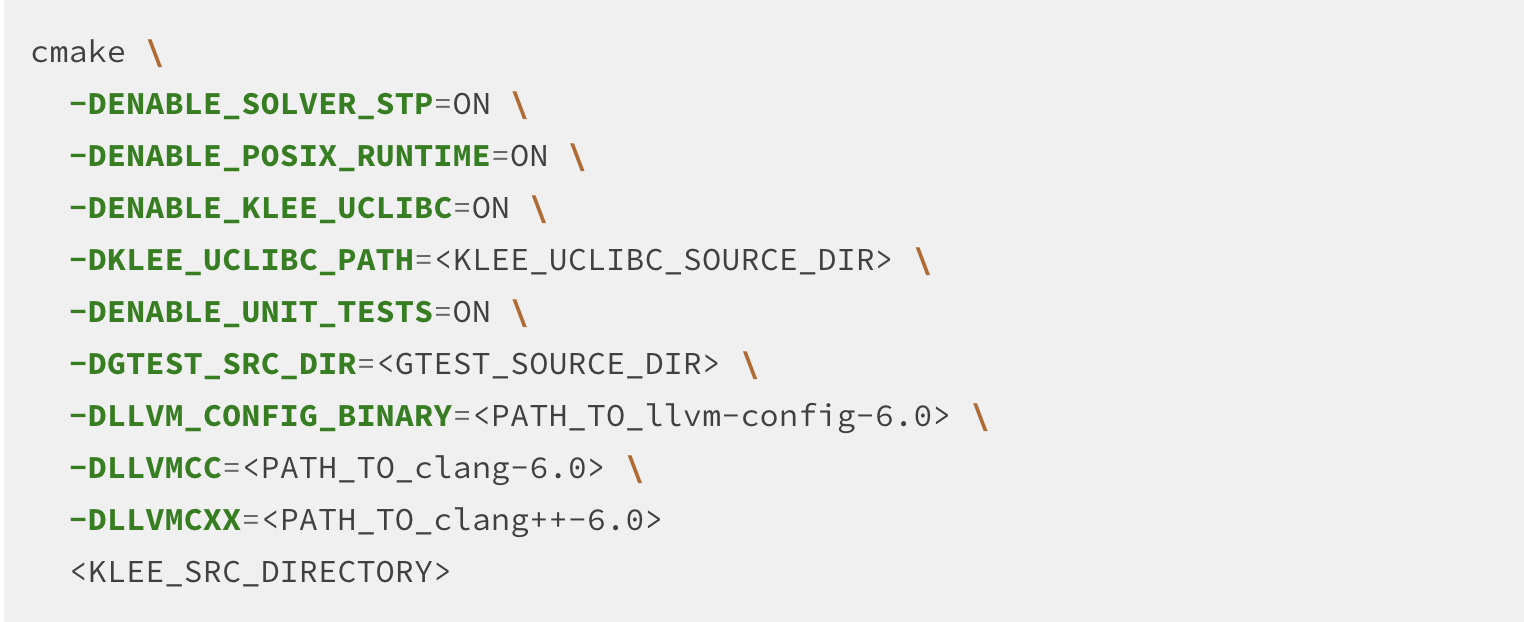
\includegraphics[scale=.3]{hinhanh/cmakeklee.png}
\end{center}
\end{figure}

Trong đó <KLEE\_UCLIBC\_SOURCE\_DIR> là đường dẫn tuyệt đối đến cây nguồn klee-uclibc, <GTEST\_SOURCE\_DIR> là đường dẫn tuyệt đối đến cây nguồn Google Test.

Bạn có thể chỉ cần nhập cmake .. thay vì như trên để sử dụng các tùy chọn mặc định cho KLEE (nhưng lưu ý rằng những điều này sẽ không bao gồm hỗ trợ cho uClibC và thời gian chạy POSIX).

Nếu không tìm thấy LLVM hoặc bạn cần sử dụng một phiên bản cụ thể, bạn có thể chuyển -DLLVM\_CONFIG\_BINARY = <LLVM\_CONFIG\_BINARY> cho CMake trong đó <LLVM\_CONFIG\_BINARY> là đường dẫn tuyệt đối đến cấu hình nhị phân phù hợp.

Tương tự, KLEE cần một trình biên dịch C và C ++ có thể tạo mã bit LLVM tương thích với phiên bản LLVM mà KLEE đang sử dụng. Nếu những điều này không được phát hiện tự động, -DLLVMCC = <PATH\_TO\_CLANG> và -DLLVMCXX = <PATH\_TO\_CLANG ++> có thể được chuyển một cách rõ ràng để đặt các trình biên dịch này, trong đó <PATH\_TO\_CLANG> là đường dẫn tuyệt đối để clang và <PATH\_TO\_CLANG ++> là đường dẫn tuyệt đối đến clang++.

Theo mặc định, KLEE sử dụng tcmalloc làm công cụ cấp phát của nó, để hỗ trợ báo cáo sử dụng bộ nhớ trên 2GB. Nếu bạn không muốn cài đặt các gói Ubuntu tcmalloc (libtcmalloc-minim4 libgoogle-perftools-dev) trên hệ thống của bạn hoặc thích sử dụng cấp phát glibc, hãy chuyển -DENABLE\_TCMALLOC = OFF sang CMake khi định cấu hình KLEE.

Cuối cùng từ thư mục build được tạo trong bước trước đó chạy lệnh sau.

\$ make

\subsubsection{Ví dụ với Klee}

Tiếp theo chúng ta sẽ tiến hành thực hiện các bước cần thiết để kiểm tra một chức năng đơn giản với KLEE. Dưới đây là function đơn giản của tôi:

\begin{figure}[ht]
\begin{center}
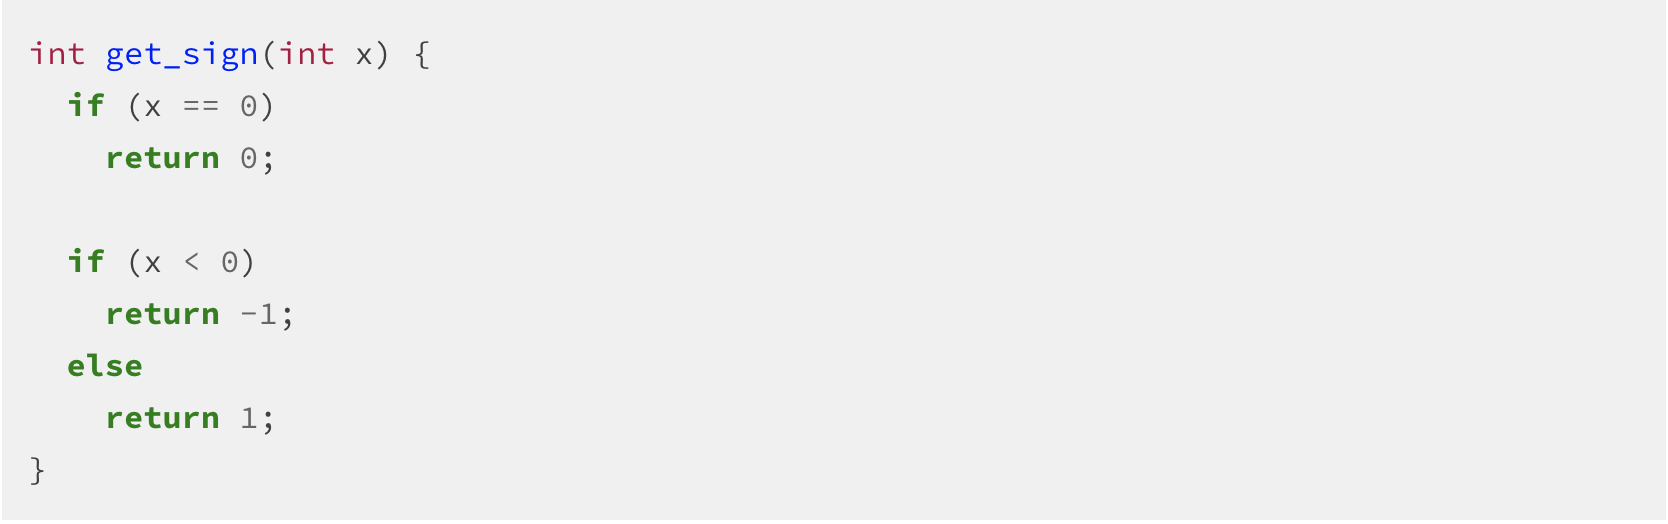
\includegraphics[scale=.3]{hinhanh/functionexample.png}
\end{center}
\end{figure}

Bời vì Klee là công cụ sinh testcase sử dung kỹ thuật Symbolic execution, nên bước tiếp theo chúng ta sẽ tạo đầu vào tượng trưng cho hàm get\_sign() ở trên.

Để kiểm tra hàm get\_sign() này với KLEE, chúng ta cần chạy nó trên đầu vào tượng trưng. Để đánh dấu một biến là tượng trưng, chúng tôi sử dụng hàm klee\_make\_symbolic() (được định nghĩa trong klee / klee.h), trong đó có ba đối số: địa chỉ của biến (vị trí bộ nhớ) mà chúng tôi muốn coi là biểu tượng, kích thước của nó và một tên (có thể là bất cứ điều gì). Dưới đây là một hàm main() đơn giản đánh dấu một biến a là ký hiệu và sử dụng nó để gọi hàm get\_sign():

\begin{figure}[ht]
\begin{center}
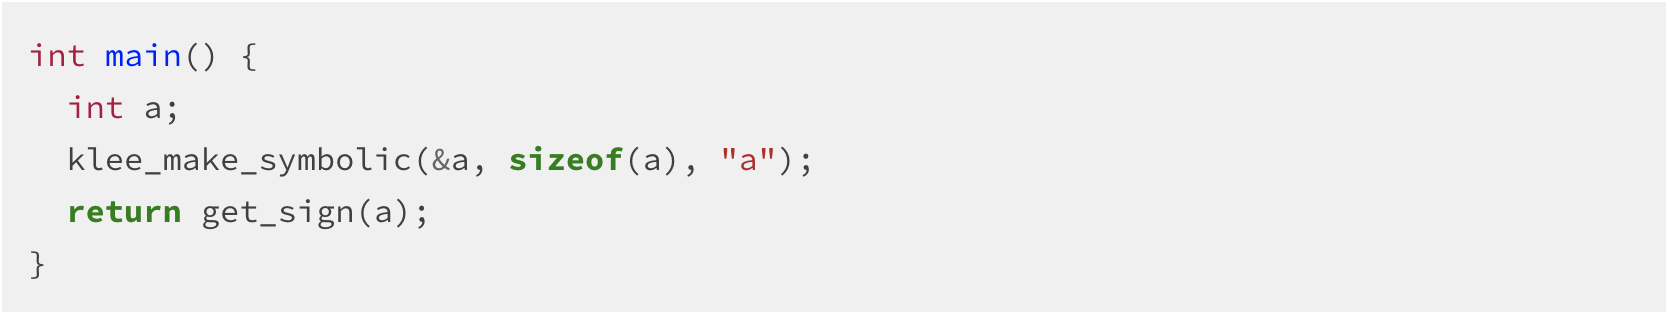
\includegraphics[scale=.3]{hinhanh/mainexample.png}
\end{center}
\end{figure}

Bước tiếp theo chúng ta sẽ tiến hành biên dịch đoạn coode bên trên thành mã bit LLVM. KLEE hoạt động trên bitcode LLVM. Để chạy một chương trình với KLEE, trước tiên bạn biên dịch nó thành mã bit LLVM bằng cách sử dụng clang -emit-llvm. Giả sử như các đoạn code bên trên được lưu trong file get\_sign.c. Từ bên trong thư mục chưa file get\_sign.c chúng ta thực hiện câu lệnh sau để biên dịch file get\_sign.c thành mã bit LLVM:

\begin{figure}[ht]
\begin{center}
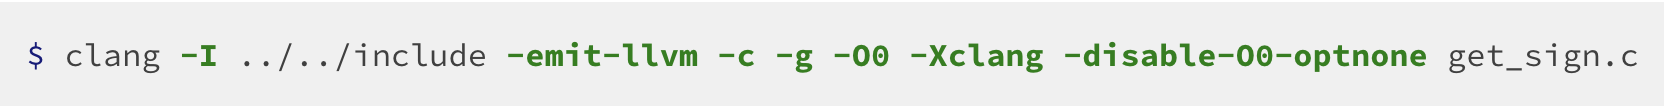
\includegraphics[scale=.3]{hinhanh/clangcompiling.png}
\end{center}
\end{figure}

Trong câu lệnh thực thi bên trên đối số -I được sử dụng để trình biên dịch có thể tìm thấy klee/klee.h, chứa các định nghĩa cho các hàm nội tại được sử dụng để tương tác với máy ảo KLEE, chẳng hạn như klee\_make\_symbolic. Rất hữu ích khi xây dựng với -g để thêm thông tin gỡ lỗi vào tệp bitcode mà chúng tôi sử dụng để tạo thông tin thống kê trên từng dòng lệnh.

Mã bit được truyền cho KLEE không nên được tối ưu hóa, bởi vì chúng tôi đã chọn thủ công các tối ưu hóa chính xác cho KLEE có thể được kích hoạt với tùy chọn dòng lệnh KLEE --optimize . Tuy nhiên, trong phiên bản sau của các phiên bản LLVM (>5.0), không nên sử dụng option -O0 khi biên dịch cho KLEE vì nó ngăn KLEE thực hiện tối ưu hóa của chính nó. Thay vào đó nên sử dụng -O0 -Xclang -disable-O0-optnone.

Nếu bạn không muốn phát lại các trường hợp thử nghiệm như được mô tả sau và không quan tâm đến thông tin gỡ lỗi và tối ưu hóa, bạn có thể xóa include klee/klee.h và sau đó biên dịch get\_sign.c với:

\begin{figure}[ht]
\begin{center}
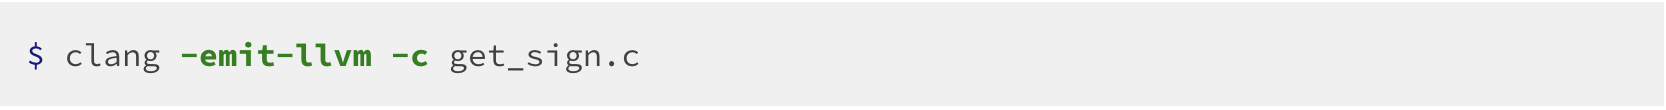
\includegraphics[scale=.3]{hinhanh/clangCompilingshort.png}
\end{center}
\end{figure}

Tuy nhiên chúng tôi vẫn khuyên bạn nên sử dụng câu lệnh dài hơn ở bên trên.

Sau khi biên dịch file get\_sign.c thành mã bit LLVM chúng ta sẽ có được file get\_sign.bc. Bước tiếp theo chúng ta sẽ tiến hành chạy file bitcode vừa được sinh ra. Để chạy KLEE trên tệp bitcode, chỉ cần thực hiện:

\begin{figure}[ht]
\begin{center}
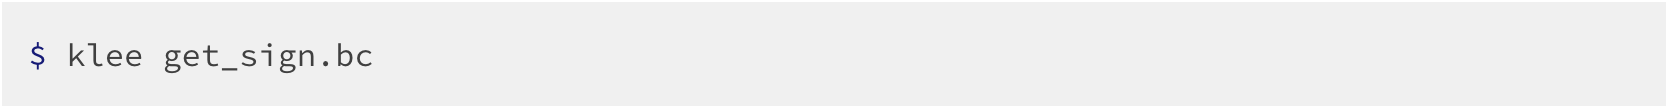
\includegraphics[scale=.3]{hinhanh/runningklee.png}
\end{center}
\end{figure}

Sau khi thực hiện xong câu lệnh ở trên bạn sẽ thấy đầu ra sau (giả sử LLVM 3.4):

\begin{figure}[ht]
\begin{center}
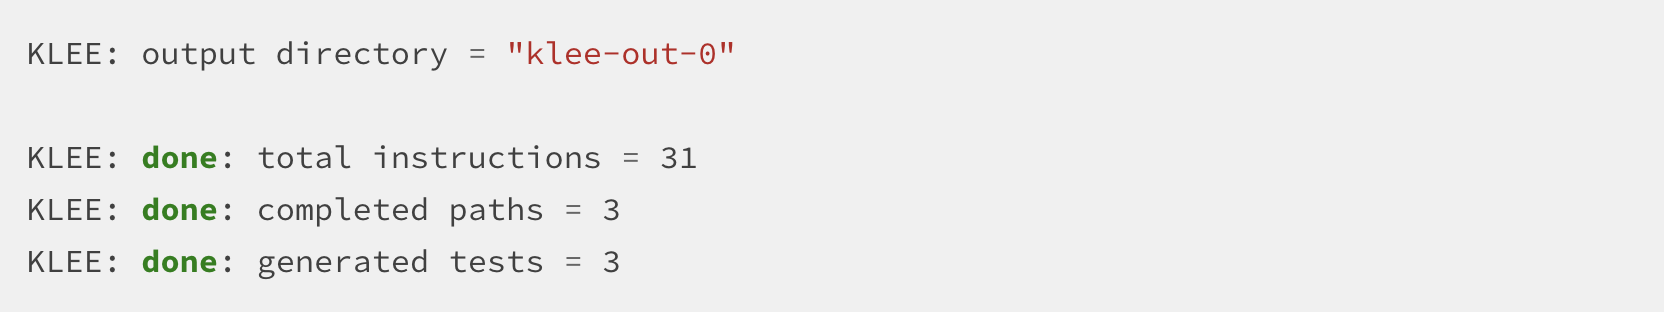
\includegraphics[scale=.3]{hinhanh/outputklee.png}
\end{center}
\end{figure}

Ở hàm get\_sign() ở trên chúng ta thấy được có  ba trường hợp thông qua chức năng bên trong hàm, một đường dẫn trong đó a bằng 0, một đường dẫn a nhỏ hơn 0 và một đường dẫn a lớn hơn 0. Như mong đợi, KLEE thông báo cho chúng tôi rằng nó đã khám phá ba đường dẫn trong chương trình và tạo ra một trường hợp thử nghiệm cho mỗi con đường khám phá. Đầu ra của một thực thi KLEE là một thư mục (trong trường hợp của chúng tôi là klee-out-0) có chứa các trường hợp thử nghiệm được tạo bởi KLEE. KLEE đặt tên cho thư mục đầu ra là klee-out-N trong đó N là số có sẵn thấp nhất (vì vậy nếu chúng ta chạy lại KLEE, nó sẽ tạo một thư mục có tên là klee-out-1) và cũng tạo ra một liên kết tượng trưng gọi là klee-last đến thư mục này cho thuận tiện:

\begin{figure}[ht]
\begin{center}
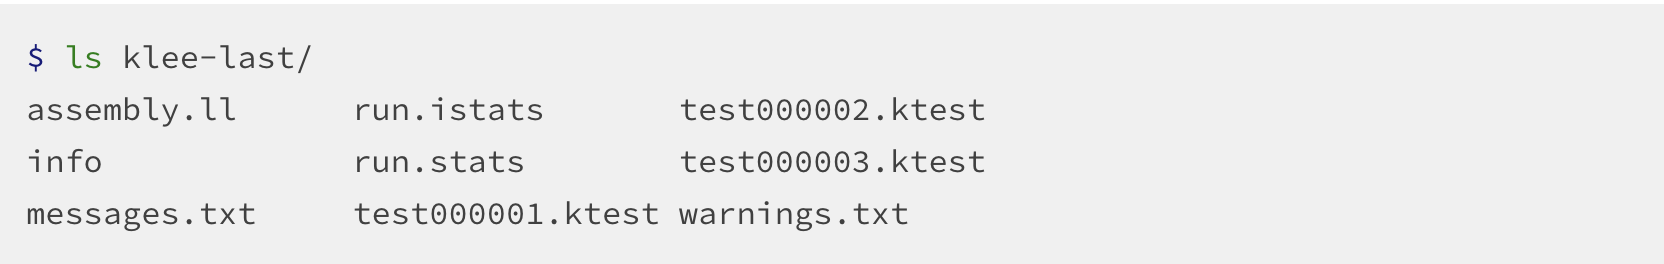
\includegraphics[scale=.3]{hinhanh/outputfolder.png}
\end{center}
\end{figure}

Dưới đây là các tệp global luôn được tạo khi thực thi Klee:

\begin{itemize}
\item[-] \textbf{Info}: Đây là một tệp văn bản chứa nhiều thông tin khác nhau liên quan đến việc chạy KLEE. Cụ thể, nó ghi lại dòng lệnh chính xác mà KLEE đã chạy và tổng thời gian thực hiện, ví dụ:

\begin{figure}[ht]
\begin{center}
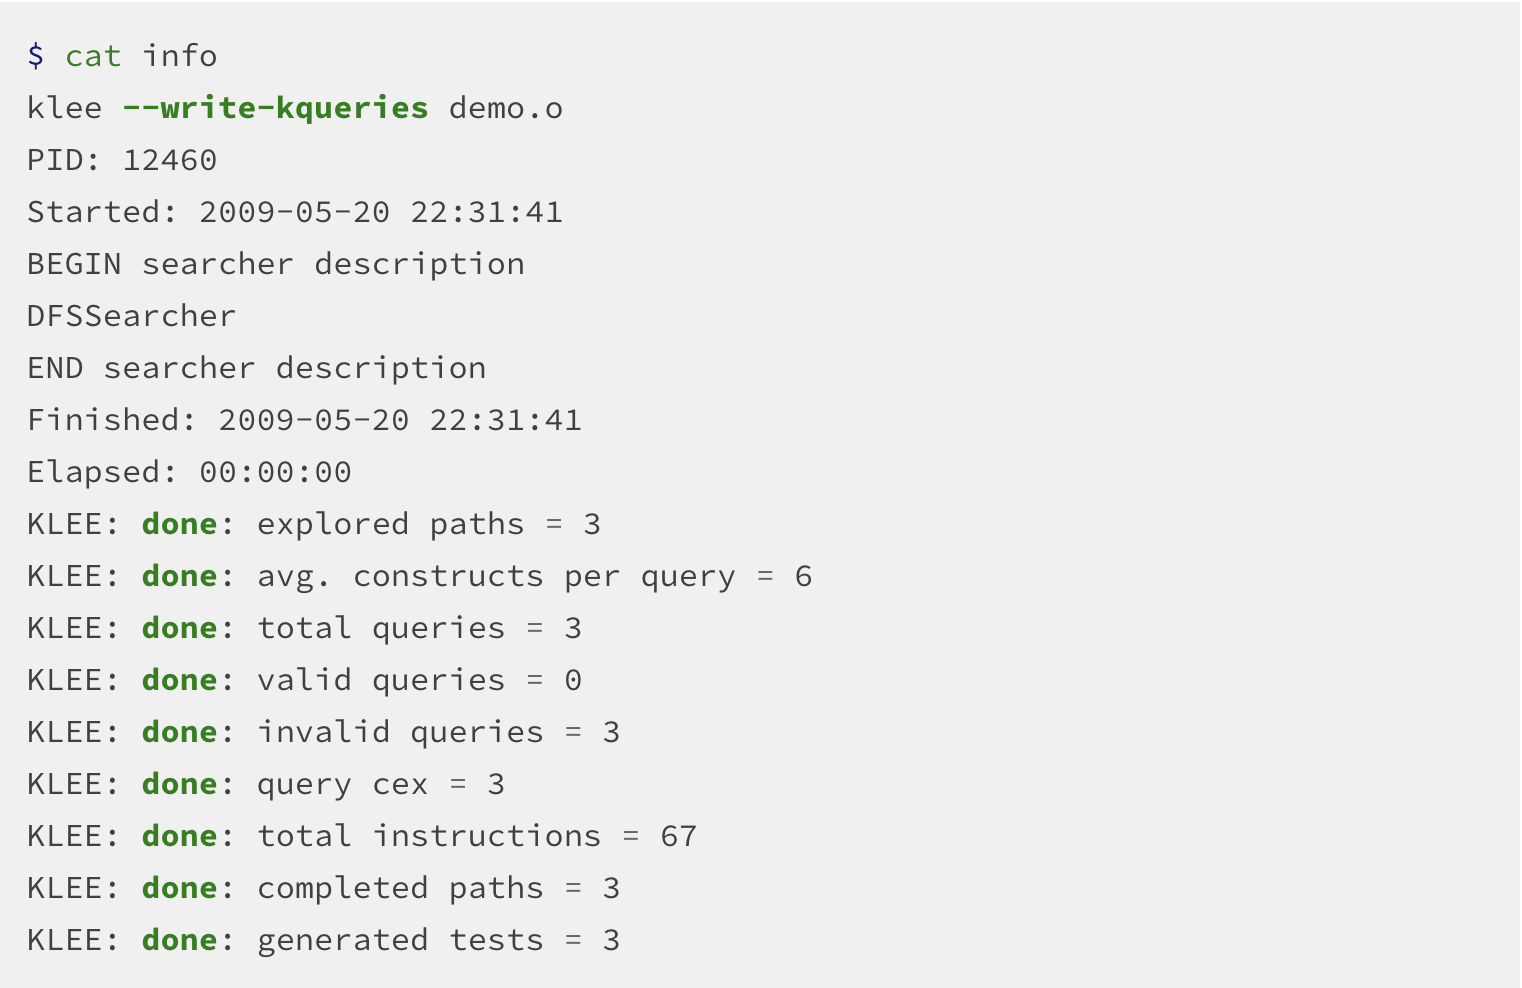
\includegraphics[scale=.3]{hinhanh/fileinfo.png}
\end{center}
\end{figure}

\item[-] \textbf{warning.txt}: Đây là tệp văn bản chứa tất cả các cảnh báo do Klee phát ra.
\item[-] \textbf{messages.txt}: Đây là một tệp văn bản chứa tất cả các tin nhắn khác được phát ra bởi Klee.
\item[-] \textbf{assembly.ll}: Tệp này chứa phiên bản con người có thể đọc được của mã bit LLVM được thực thi bởi Klee. 
\item[-] \textbf{run.stats}: Đây là một tệp văn bản chứa các số liệu thống kê khác nhau được phát ra bởi Klee.
\item[-] \textbf{run.istats}: Đây là một tệp nhị phân chứa số liệu thống kê toàn cầu do KLEE phát ra cho mỗi dòng mã trong chương trình.
\end{itemize}

Ngoài ra còn có các file được tạo ra dựa trên các trường hợp:

\begin{itemize}
\item[-] \textbf{test<N>.ktest}: Chứa thông tin bộ testcase thử nghiệm được tạo bởi Klee trên các trường hợp. Sử dụng công cụ ktest để đọc nội dung. Việc tạo các tệp .ktest có thể bị vô hiệu hóa bằng cách sử dụng tùy chọn --no-output.
\item[-] \textbf{test<N>.<error-type>.err}: Được tạo cho các  hợp trong đó Klee tìm thấy lỗi. Chứa thông tin về lỗi ở dạng văn bản.
\item[-] \textbf{test<N>.kquery}: Chứa các ràng buộc liên quan đến trường hợp đã cho, theo định dạng KQuery. Việc tạo các tệp này có thể được kích hoạt thông qua cờ --write-kqueries.
\item[-] \textbf{test<N>.cvc}: Chứa các ràng buộc liên quan đến trường hợp đã cho, ở định dạng CVC. Việc tạo các tệp này có thể được kích hoạt thông qua cờ --write-cvcs. (Đây là thông tin giống như trong tệp .kquery tương ứng.)
\item[-] \textbf{test<N>.smt2}: Chứa các ràng buộc liên quan đến trường đã cho, ở định dạng SMT-LIBv2. Việc tạo các tệp này có thể được kích hoạt thông qua cờ --write-smt2s. (Đây là thông tin giống như trong tệp .kquery tương ứng.)
\end{itemize}

Sau khi đã tìm hiểu về các file chứa trong output khi thực thi file bitcode chúng ta cùng xem các trường hợp đã được tạo ra của klee. Các trường hợp thử nghiệm được tạo bởi Klee được ghi vào các tệp có phần mở rộng .ktest. Đây là các tệp nhị phân có thể được đọc với hàm tiện ích ktest-tool. ktest-tool đưa ra các cách biểu diễn khác nhau cho cùng một đối tượng, ví dụ chuỗi byte Python (dữ liệu), số nguyên (int) hoặc văn bản ascii (văn bản). Chúng ta hãy kiểm tra từng file có phần mở rộng .ktest đã được tạo ra ở phần trên:

\begin{figure}[ht]
\begin{center}
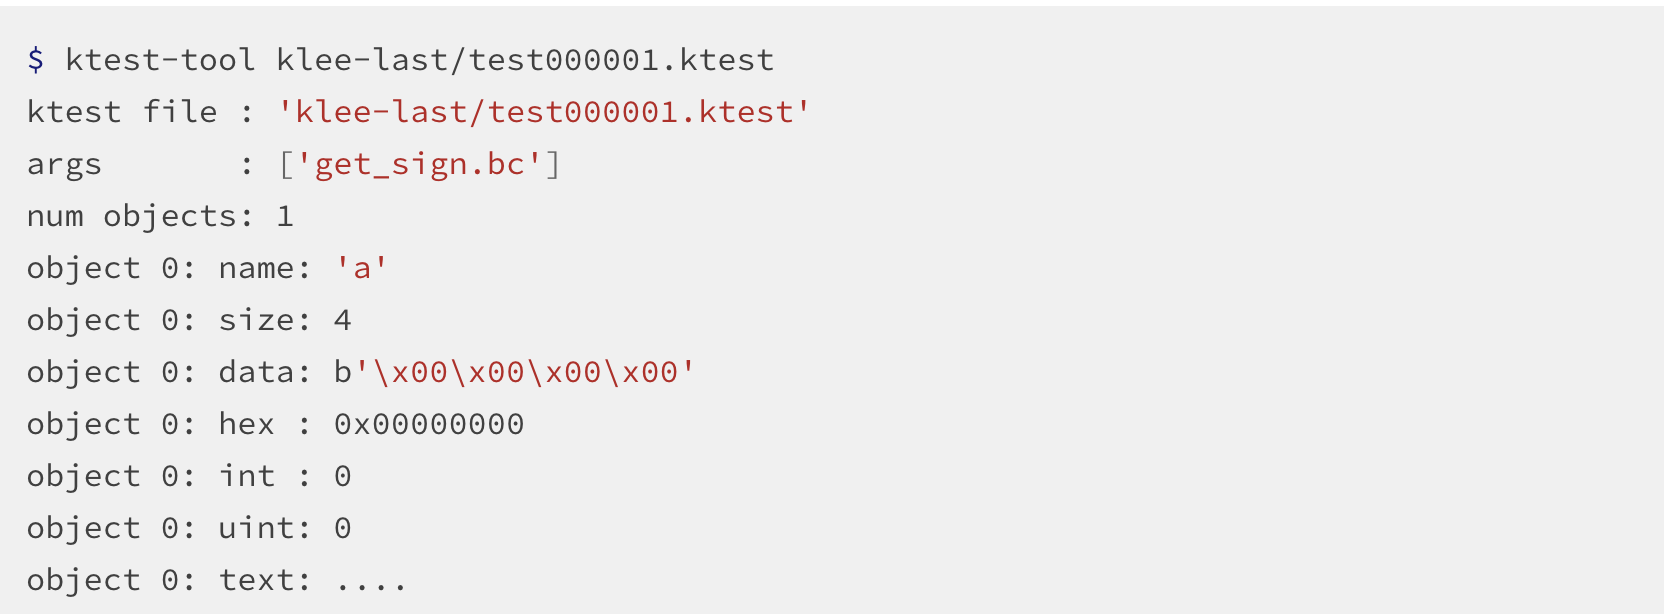
\includegraphics[scale=.3]{hinhanh/test1.png}
\end{center}
\end{figure}

\begin{figure}[ht]
\begin{center}
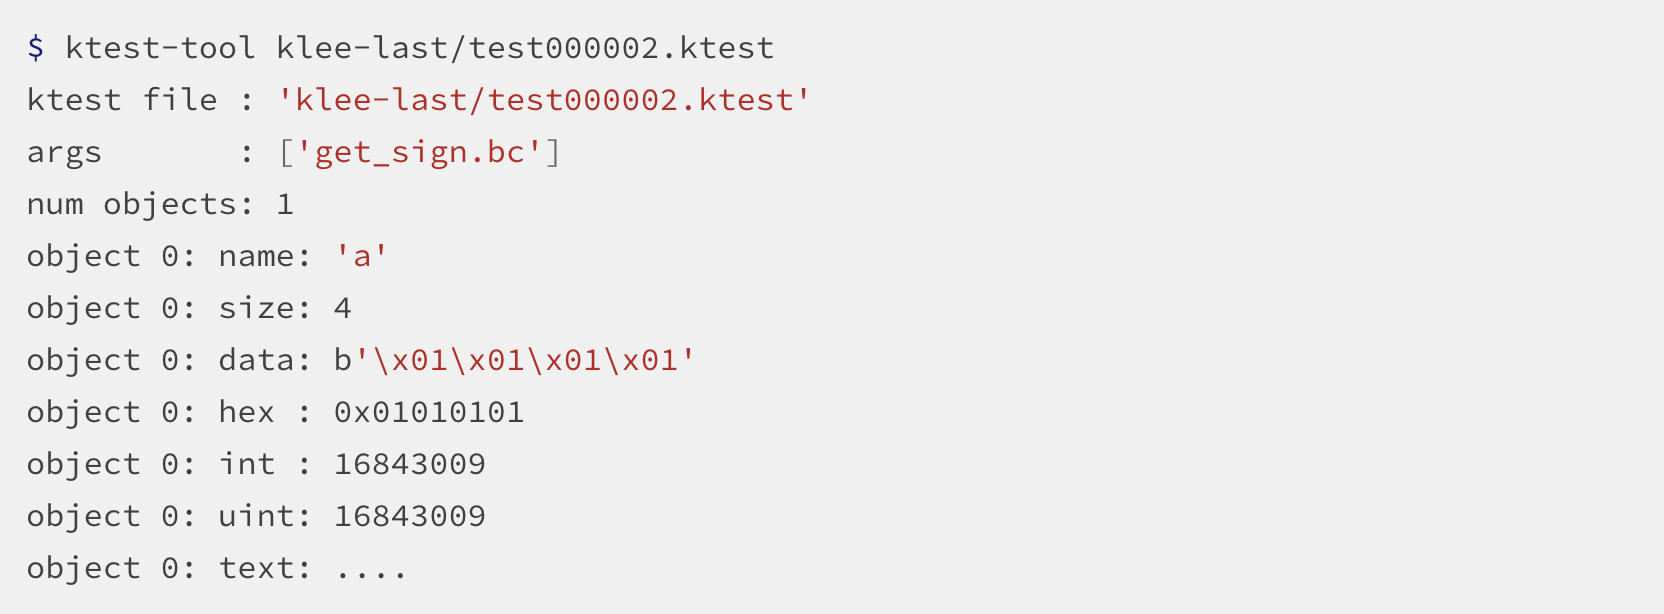
\includegraphics[scale=.3]{hinhanh/test2.png}
\end{center}
\end{figure}

\begin{figure}[ht]
\begin{center}
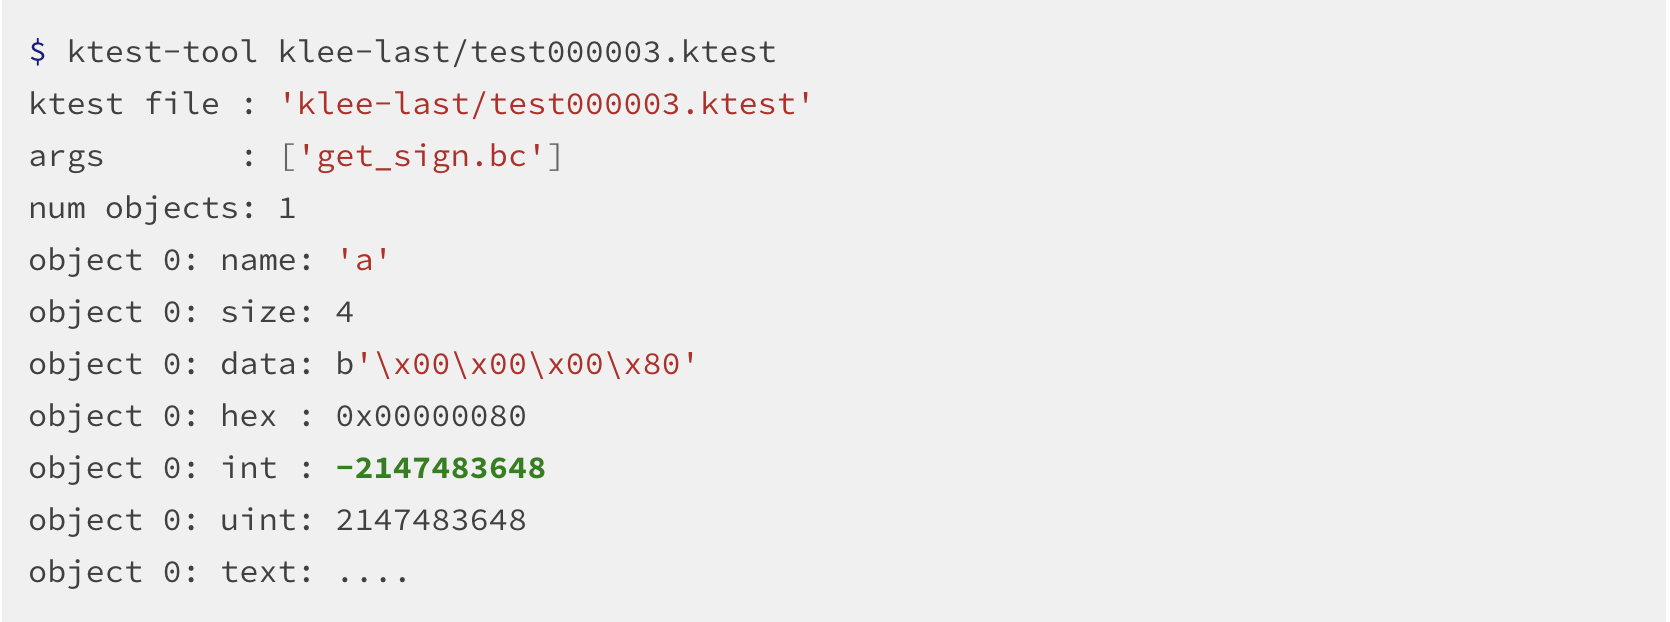
\includegraphics[scale=.3]{hinhanh/test3.png}
\end{center}
\end{figure}

Trong mỗi tệp kiểm tra, KLEE báo cáo các đối số mà chương trình được gọi (trong trường hợp của chúng tôi không có đối số nào ngoài tên chương trình), số lượng đối tượng tượng trưng trên đường dẫn đó (chỉ có một trong trường hợp của chúng tôi), tên của biểu tượng của chúng tôi đối tượng ('a') và kích thước của nó (4). Bản thân thử nghiệm thực tế được biểu thị bằng giá trị đầu vào của chúng tôi: 0 cho thử nghiệm đầu tiên, 16843009 cho thử nghiệm thứ hai và -2147483648 cho thử nghiệm cuối cùng. Như mong đợi, KLEE tạo ra giá trị 0, một giá trị dương (16843009) và một giá trị âm (-2147483648). Bây giờ chúng tôi có thể chạy các giá trị này trên phiên bản gốc của chương trình để thực hiện tất cả các trường hợp thông qua mã.

Sau khi đã có được các testcase chúng ta sẽ thay vào trong hàm get\_sign() để có được kết quả. Mặc dù tôi có thể chạy các trường hợp thử nghiệm do KLEE tạo ra trên chương trình của chúng tôi bằng tay, (hoặc với sự trợ giúp của cơ sở hạ tầng kiểm tra hiện có), Klee cung cấp một thư viện phát lại thuận tiện, chỉ cần thay thế cuộc gọi đến klee\_make\_symbolic bằng một cuộc gọi đến chức năng gán để đầu vào của chúng tôi giá trị được lưu trữ trong tệp .ktest. Để sử dụng nó, chỉ cần liên kết chương trình của bạn với thư viện libkleeRuntest và đặt biến môi trường KTEST\_FILE để trỏ đến tên của trường hợp thử nghiệm mong muốn:

\begin{figure}[ht]
\begin{center}
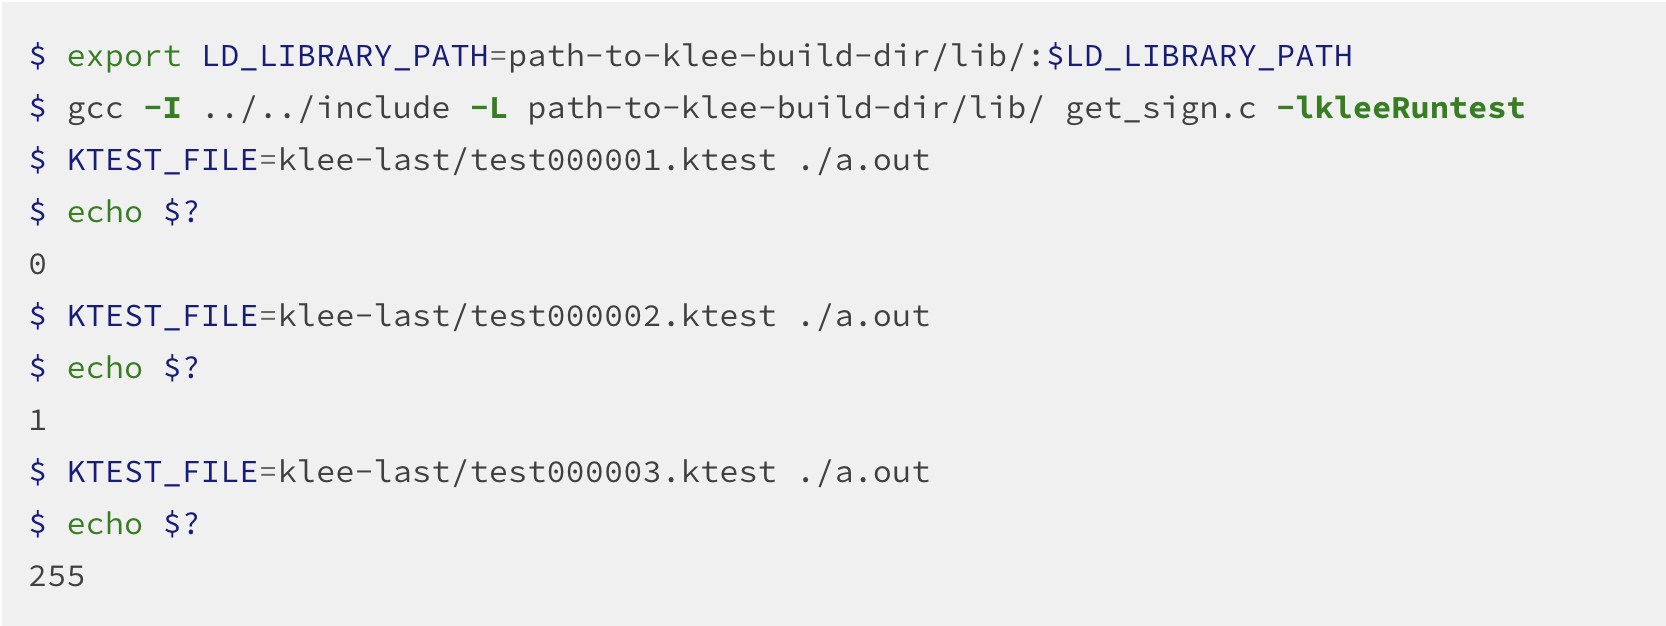
\includegraphics[scale=.3]{hinhanh/replayingtestcase.png}
\end{center}
\end{figure}

Như mong đợi, chương trình của chúng tôi trả về 0 khi chạy trường hợp thử nghiệm đầu tiên, 1 khi chạy trường hợp thứ hai và 255 (-1 được chuyển đổi thành giá trị mã thoát hợp lệ trong phạm vi 0-255) khi chạy trường hợp cuối cùng.

\subsubsection{Hàm tự sinh testcase}
Như ở phần trên chúng ta đã tiến hành sinh testcase tự động với công cụ Klee. Đối với hàm get\_sign() ở phần trên tham số đầu vào của hàm chỉ là 1 số nguyên nên trong quá trình chạy thử nghiệm chúng ta đã nhận được kết quả đúng như mong muốn.  Đối với những hàm có tham số đầu vào phức tạp hơn, ví dụ như là một array có số phần tử là n thì Klee chưa tạo ra các bộ test case như  mong muốn. Ta xét ví dụ bên dưới:

\begin{lstlisting}[language=c]
int lon_nhi(int arr[], int n)
{
  int temp = 0, largest1 = 0, largest2 = 0;
  largest1 = arr[0];
  largest2 = arr[1];
  if (largest1 < largest2)
  { 
    temp = largest1;
    largest1 = largest2;
    largest2 = temp;
  }
  
  for (int i = 2; i < n; i++)
  { 
    if (arr[i] > largest1)
    {   
        largest2 = largest1;
        largest1 = arr[i];
    }
    else if (arr[i] > largest2 && arr[i] != largest1)
    {   
        largest2 = arr[i];
    }
  }
  return largest2;
}
\end{lstlisting}

Đối với hàm lon\_nhi() với tham số đầu vào là một array và một số nguyên n, Klee không tạo ra được những bộ testcase như mọng đợi. Sau khi được biên dịch thành file bitcode, tôi tiến hành chạy file bitcode để có được output.

\begin{figure}[ht]
\begin{center}
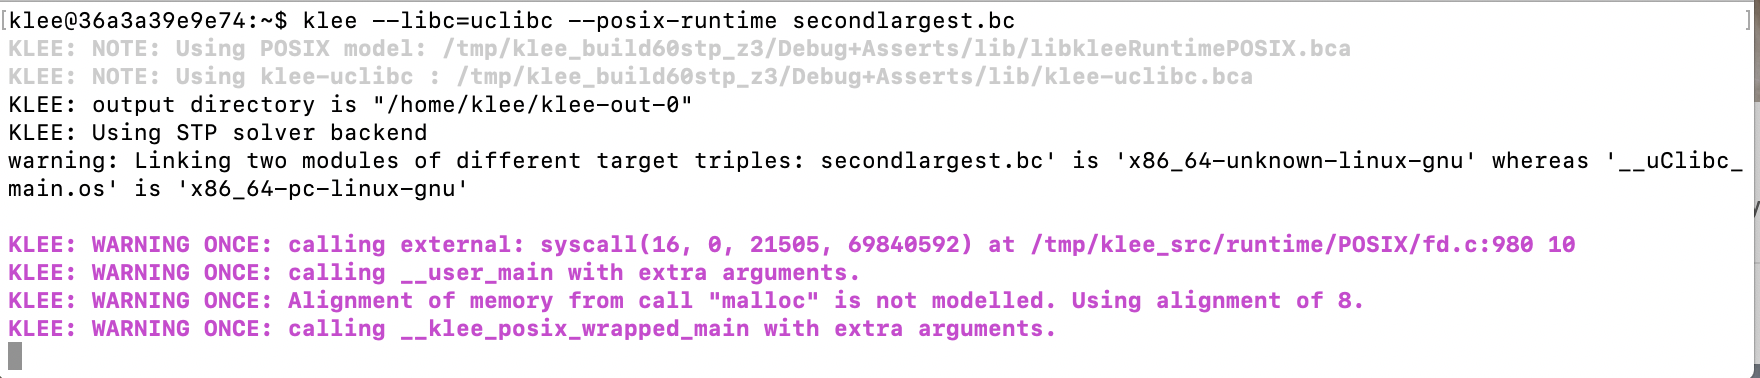
\includegraphics[scale=.3]{hinhanh/runningkleearray.png}
\end{center}
\end{figure}

Nhưng khi tiến hành chạy file bitcode như hình trên thì quá trình sinh test diễn ra liên tục và không kết thúc. 

Để giải quyết vấn đề trên thì tôi tiên hành viết một hàm tự động sinh test ngẫu nhiên để có thể tạo ra các bộ testcase cho các bài tập có các tham số đầu vào là array. Hàm này sẽ được chạy đầu tiên trong công cụ chấm điểm để có thể tạo ra bộ các testcase cho phần chấm điểm bài lập trình.

\begin{lstlisting}[language=c]
void printRandoms(int lower, int upper, int count, FILE *out) 
{ 
    int i;
    fprintf(out,"%d\n",count);
    for (i = 0; i < count; i++) { 
        int num = (rand() % (upper - lower + 1)) + lower; 
        fprintf(out,"%d ",num); 
    }
    fprintf(out,"\n"); 
} 

int randomNumber(int lower, int upper)
{
    int num = (rand() % (upper - lower + 1)) + lower; 
    return num;
}

void setup(int lower, int upper, int n, FILE *out)
{
    int count;
    fprintf(out,"%d\n",n);
    srand(time(0)); 
    for(int i = 0; i < n; i++)
    {
        count = randomNumber(0, 10);
        printRandoms(lower, upper, count, out);
    } 
    fclose(out);
}
\end{lstlisting}

Hàm setup() bên trên có 4 tham số đầu vào, trong đó lower và upper dùng để giới hạn giá trị các phần tử trong mảng phải lớn hơn hoặc bằng lower và nhỏ hơn hoặc bằng upper. Tham số n dùng để giới hạn số bộ test được sinh ra. Con trỏ *out dùng để ghi kết quả các bộ testcase sinh được ra file text. Bên trong hàm setup() sẽ gọi 2 hàm con là hàm randomNumber() dùng để tạo ra sô phần tử trong một array và hàm printRandoms() dùng để sinh ra các bộ testcase tương ứng với số phần tử là giá trị của hàm randomNumber(). Các bộ testcase được sinh ra sẽ được ghi vào trong 1 file output với giá trị của dòng đầu tiên là số lượng các bộ testcase được sinh ra và các dòng tiếp theo sẽ là các bộ testcase.
Sau khi có được file output công cụ sẽ tiến hành chấm điểm bài tập lập trình dựa trên các bộ testcase chứa trong file output đó.

\subsection{Cách ra đề bài}
Khi giáo viên tiến hành tạo đề bài sẽ tạo trước cho sinh viên một function prototype, function prototype này thể hiện tên của function sinh viên cần hoàn thành và các tham số đầu vào của function này. Nhiệm vụ của sinh viên là đọc hiểu để bài và hoàn thành nội dung bên trong của function.

Cùng tìm hiểu qua ví dụ sau đây:

Đề bài: Cho một mãng số nguyên có n phần tử. Sắp xếp mãng số nguyên đó theo thứ tự tăng dần.

Ví dụ: Nếu cho một mãng sau arr = [3, 1, 7, 10, 2, 14], và sau khi được sắp xếp mãng đó sẽ trở thành arr = [1, 2, 3, 7, 10, 14].

Định dạng đầu vào: Đầu vào của chương trình sẽ được chứa trong 1 file có phần mở rộng là .txt. Dòng đầu tiên chứa một số nguyên n sẽ biểu thị kích thước của mãng. Dòng tiếp theo chứa các số nguyên là phần tử của mãng được phân tách với nhau bằng dấu cách.

Các ràng buộc:

\begin{itemize}
\item[-] 1 <= n <= 1000
\item[-] 1 <= arr$_{i}$  <= 1000, trong đó arr$-{i}$ là phần tử thứ i$^{th}$ của mãng.
\end{itemize}

Định dạng đầu ra: Kết quả sau khi được xử lý sẽ là một mãng đã được sắp xếp theo thứ tự tăng dần và mãng đó được ghi vào trong file output có phần mở rộng là .txt.

Input mẫu:

\begin{figure}[ht]
\begin{center}
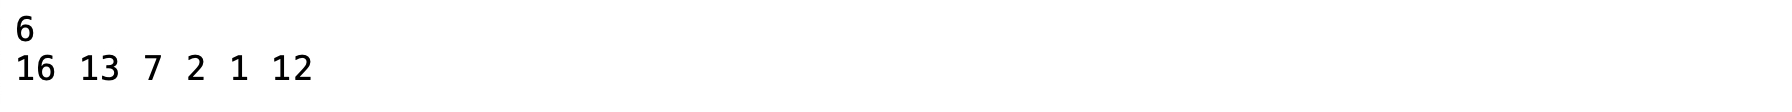
\includegraphics[scale=.3]{hinhanh/inputsample.png}
\end{center}
\end{figure}

Output mẫu:

\begin{figure}[ht]
\begin{center}
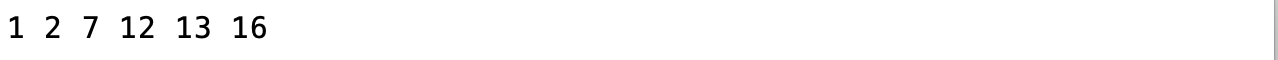
\includegraphics[scale=.3]{hinhanh/outputsample.png}
\end{center}
\end{figure}

Function prototype mẫu:

\begin{lstlisting}[language=c]
void sapXep(int a[100], int n);

int main() {
    int arr[100], n;
    FILE *inp, *out;

    if ((inp = fopen("./datatest/test.txt", "r")) == NULL)
    {
        printf("Error! opening file");
        exit(1);         
    }
    fscanf(inp,"%d", &n);

    for(int i = 0; i < n; i++) {
        fscanf(inp,"%d", &arr[i]);
    }
    fclose(inp);

    sapXep(arr,n);

    if ((out = fopen("out.txt", "w")) == NULL)
    {
        printf("Error! opening file");
        exit(1);         
    }

    for(int j = 0; j < n; j++) {
        fprintf(out,"%d ",arr[j]);
    }
    fclose(out);
}
\end{lstlisting}

Như đoạn code phía trên, sinh viên chỉ cần đọc hiểu yêu cầu đề bài và hoàn thành hàm sapXep() ở phía trên mà không cần quan tâm phía trong hàm main làm gì. Chương trình đã tự động gọi hàm sapXep và ghi lại kết quả của hàm sapXep() ra file output.

\subsection{Cách chấm điểm}
Sau khi đã thực thi chương trình chấm điểm chúng ta sẽ thu được kết quả là số bộ testcase cho ra kết quả chính xác và số bộ testcase cho ra kết quả không chính xác theo bài tập lập trình của sinh viên. Dựa vào kết quả thu được ta sẽ tính ra được số điểm của sinh viên theo công thức sau:

Số điểm =$\frac{ 10 }{ Tong so bo testcase }$ * So bo testcase dung

Ví dụ: Chương trình có 10 bộ testcase, sau khi thực thi kết thúc và thu được 7 bộ testcase cho kết quả chính xác thì số điểm của sinh viên là (10 / 10) * 7 = 7 điểm.

\section{Thực nghiệm}

\subsection{Bài tập với đầu vào là các kiểu dữ liệu nguyên thủy}

Đề bài: Cho 3 số nguyên ngẫu nhiên. Tìm số có giá trị lớn nhất trong 3 số.

Ví dụ: Nếu cho a = 5, b = 5, c = 3, sau khi thực thi xong sẽ cho ra giá trị lớn nhất là 5.

Trước khi đi vào chạy thực nghiệm, chúng ta sẽ đi qua tìm hiểu về cách tổ chức thư mục chứa các file dùng để thực thi khi tiến hành thực nghiệm.

\begin{figure}[ht]
\begin{center}
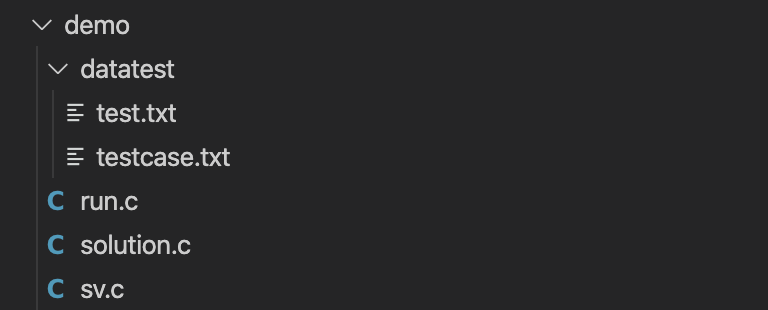
\includegraphics[scale=.3]{hinhanh/cautrucfolder.png}
\end{center}
\end{figure}

Như hình bên trên trong thư mục demo sẽ chưa toàn bộ các file và thư mục cần thiết để thực thi chương trình. Trong thư mục demo có 2 file là test.txt và testcase.txt. File testcase.txt sẽ chứa thông tin tổng số bộ test cần thực hiện và các bộ test cần thực hiện. Và cứ mỗi lần thực hiện kiểm tra bộ test chương trình sẽ tiến hành ghi bộ từng bộ test ra file test.txt.

\begin{figure}[ht]
\begin{center}
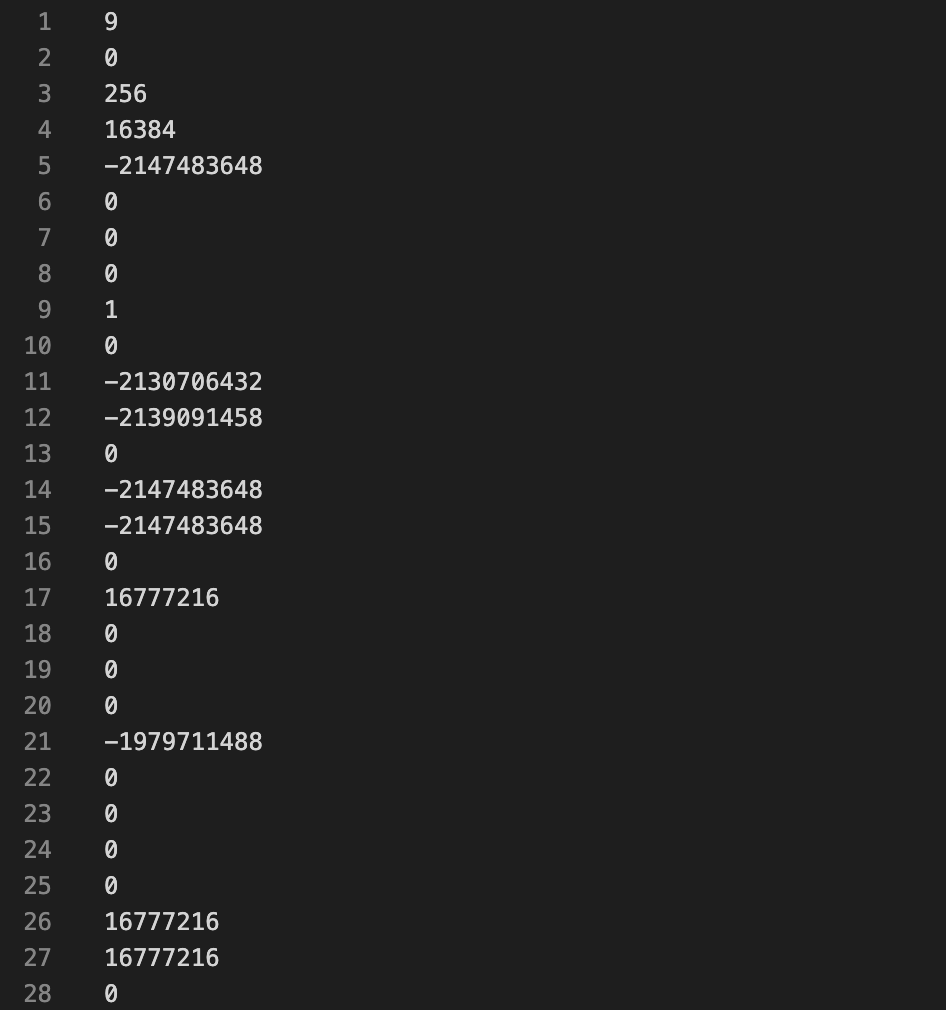
\includegraphics[scale=.3]{hinhanh/testcase.png}
\end{center}
\end{figure}

Như hình bên dưới thì dòng đầu tiên sẽ biểu hiện tổng số bộ testcase. Các dòng tiếp theo sẽ là các bộ testcase. Ở trong file này cứ 3 dòng liên tiếp sẽ ứng với 1 bộ testcase để ứng với 3 input đầu vào của để bài trên. Với mỗi lần thực hiện chương trình sẽ đọc thông tin ở 3 dòng liên tiếp (trừ dòng đầu tiên) để ghi sang file test.txt là input cho mỗi lần chạy chương trình.

Tiếp theo là file solution.c, file này chứa code bài giải của đề bài ở trên, thông thường code trong file này là do giáo viên (hoặc người ra đề) tạo ra. File này sẽ tiến hành đọc dữ liệu từ file test.txt để lấy làm input đầu vào và tiến hành thực thi. Sau khi thực thi thành công sẽ cho ra 1 file output là out.txt chứa kết quả trả về sau khi thực thi của chương trình.

Tương tự như file solution.c là file sv.c, file này cũng chứa code bài giải của đề bài ở trên. Nhưng khác với solution.c file sv.c là do sinh viên làm và nộp lại. File này cũng tiến hành đọc dữ liệu từ file test.txt để lấy làm input đầu vào và tiến hành thực thi. Sau khi thực thi thành công sẽ cho ra 1 file output là outsv.txt chứa kết quả trả về sau khi thực thi của chương trình.

Cuối cùng là file run.c, file này là file chính để tiến hành chấm điểm cho bài tập lập trình của sinh viên. Đầu tiên chương trình sẽ tiến hành đọc dữ liệu từ file testcase.txt để có được số lượng tổng bộ testcase cần thực hiện. Sau khi có được tổng số bộ testcase chương trình sẽ tiếp hành việc chấm điểm bài tập lập trình của sinh viên bằng cách so sánh kết quả của 2 file solution.c và sv.c. Dựa trên tổng số bộ testcase mà chương trình sẽ lặp với số lần tương ứng, mỗi lần lặp như vậy chương trình sẽ đọc 1 bộ testcase từ file testcase.txt để ghi ra file test.txt. Sau khi bộ test đã được ghi ra file test.txt, 2 file solution.c và sv.c sẽ tiến hành đọc bộ test được ghi trong file test.txt để thực hiện và cho ra output là 2 file out.txt và outsv.txt. Sau khi có được 2 file output chương trình sẽ tiến hành kiểm tra kết quả trong 2 file output có giống nhau hay không. Sau khi kết thúc vòng lặp chúng ta sẽ thu được số bộ test đúng và số bộ test không đúng. Dựa vào kết quả thu được chương trình sẽ tính được điểm của sinh viên (cách tính điểm tôi đã có đề cập trong phần "Cách chấm điểm" ở trên.

Trường hợp đầu tiên tôi sẽ tiến hành chấm điểm có bài tập của sinh viên chưa đúng trong một số bộ testcase. Cùng xem qua cách giải quyết của sinh viên sau:

\begin{lstlisting}
int max(int a, int b, int c)
{
  if(a > b && a >c){   
    return a;
  } else if(b >a && b >c){
    return b;
  } else {
    return c;
  }
}
\end{lstlisting}

Cùng xem qua đoạn mã thực hiện chấm điểm sau:

\begin{lstlisting}
int main ()
{
   FILE *inp,*out;
   int n,a,b,c, wrong, success;
   float diem;
   success = 0;
   wrong = 0;
   if ((inp = fopen("./datatest/testcase.txt", "r")) == NULL)
   {
      printf("Error! opening file");
      exit(1);         
   }
   fscanf(inp,"%d",&n);
   for(int i = 0; i < n; i++) {
      if((out = fopen("./datatest/test.txt", "w")) == NULL)
      {
         printf("Error! opening file");
         exit(1);         
      }
      printf("Test lan thu %d\n", i + 1);
      fscanf(inp,"%d",&a);
      fscanf(inp,"%d",&b);
      fscanf(inp,"%d",&c);
      fprintf(out,"%d\n",a);
      fprintf(out,"%d\n",b);
      fprintf(out,"%d\n",c);
      fclose(out);
      char commandSolution[50],commandRunSolution[50],commandSV[50];
      char commandRunSV[50],commandCompare[50];

      strcpy(commandSolution, "gcc -Wall -o solution solution.c" );
      strcpy(commandSV, "gcc -Wall -o sv sv.c" );
      strcpy(commandRunSolution, "./solution");
      strcpy(commandRunSV, "./sv");
      strcpy(commandCompare, "diff ./out.txt ./outsv.txt");
      system(commandSolution);
      system(commandSV);
      system(commandRunSolution);
      system(commandRunSV);

      if(system(commandCompare) == 0) {
         printf("succcessful\n");
         success = success + 1;
      }else {
         //diem = diem - 1.5;
         wrong = wrong + 1;
         printf("wrong\n");
         printf("Bo test case: a = %d, b = %d, c = %d\n", a,b,c);
      }
   }
   fclose(inp);
   diem = (10.0 / n) * success;
   printf("So bo testcase sai: %d\n", wrong);
   printf("Diem cua ban la: %.2f\n", diem);
   return(0);
}
\end{lstlisting}

Trong đoạn code trên tôi sử dụng hàm fopen() để đọc ghi file, tham số đầu tiền sẽ là đường dẫn đích đến file cần đọc/ghi, tham số thứ hai dùng để truy cập đến chế độ cần sử dụng (đọc hoặc ghi file,...).

Ví dụ: hàm fopen("./datatest/testcase.txt", "r") sẽ tiến hành truy cập vào file testcase.txt để đọc dữ liệu.

Sau khi dọc dữ liệu từ testcase.txt và ghi dữ liệu vào file test.txt chương trình sẽ thực thi các câu lệnh hệ thống để biên dịch các file có phần mở rộng là .c. Sau khi đã biên dịch xong sẽ sử dụng file output của quá trình biên dịch để chạy chương trình. Như ở trên thì tôi sử dụng hàm system() để có thể thực thi các lệnh hệ thống trong C.

Khi chạy xong các file biên dịch, chương trình sẽ cho ra 2 file output kết quả. Để biết là bài tập sinh viên có chạy đúng với bộ tetscase tương ứng hay không tôi sử dụng lệnh diff để kiểm tra sự khác biệt của 2 file output.

Sau khi đã tiến hành kiểm tra hết tất cả bộ testcase, chương tình sẽ tính  được điểm của sinh viên dựa trên số bộ testcase đúng và số bộ testcase không đúng.

Cùng xem qua quá trình chạy thực nghiệm đối với đề bài ở trên:

Đầu tiên tôi tiến hành biên dịch file run.c trước khi chạy.

\begin{figure}[ht]
\begin{center}

\includegraphics[scale=.3]{hinhanh/compilerdemo.png}
\end{center}
\end{figure}

Sau khi compiler thành công trong thư mục sẽ xuất hiện thêm file run.

\begin{figure}[ht]
\begin{center}
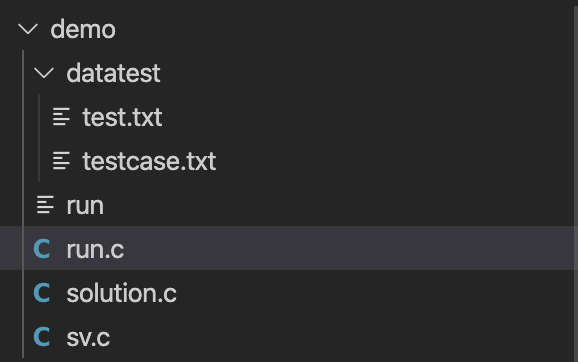
\includegraphics[scale=.3]{hinhanh/cautrucsaucompiler.png}
\end{center}
\end{figure}

Để có thể chạy chương tình chúng ta tiến hành chạy file run vừa được tạo ra.

\begin{figure}[ht]
\begin{center}

\includegraphics[scale=.3]{hinhanh/rundemo.png}
\end{center}
\end{figure}

Kết quả khi chạy file run để chấm điểm.

\begin{figure}[ht]
\begin{center}
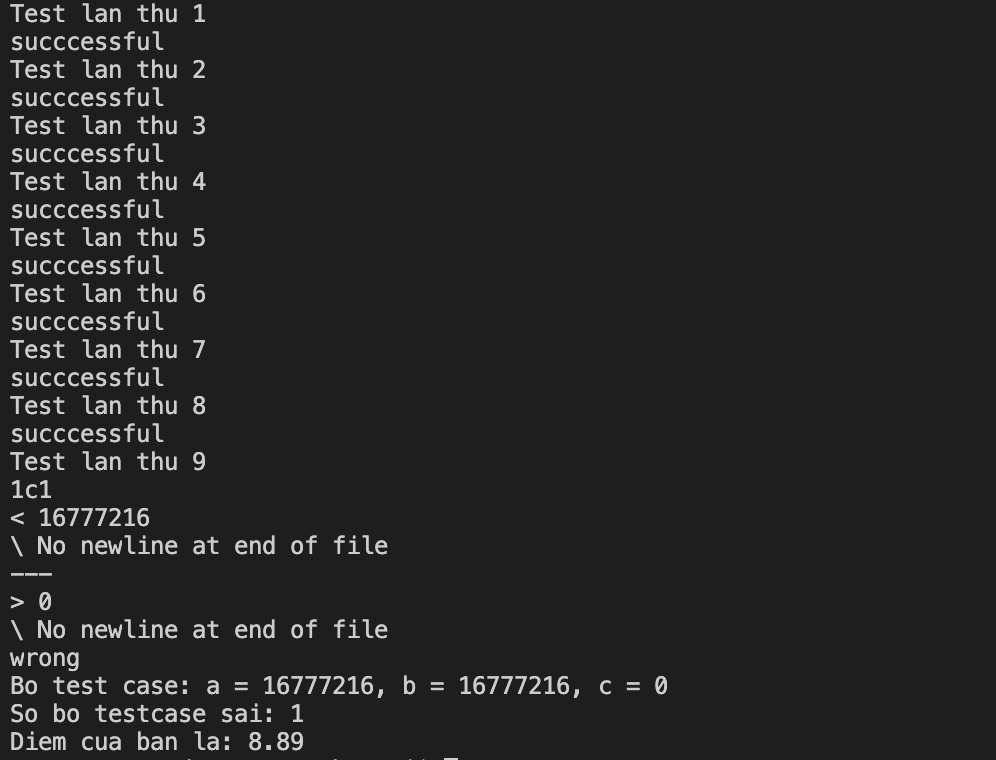
\includegraphics[scale=.3]{hinhanh/ketquademo.png}
\end{center}
\end{figure}

Như hình bên trên chúng ta thấy chương trình có tất cả 9 bộ test. Khi chạy đến bộ test thứ 9 thì bài của sinh viên cho ra kết  quả không đúng với bộ test đầu vào a = 16777216, b = 16777216, c = 0. Trong khi kết quả của solution cho ra là 16777216 thì bài của sinh viên lại cho ra kết quả là 0. Sau khi chạy hết tất cả các bộ test chương chình sẽ thông báo số bộ test không đúng của sinh viên là 1 và điểm số của sinh viên là 8.89đ.

Cùng xem lại thư mục sau khi chạy xong file run.

\begin{figure}[ht]
\begin{center}
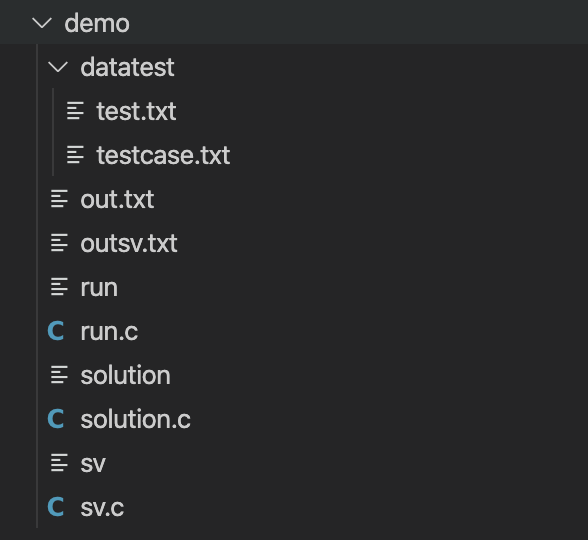
\includegraphics[scale=.3]{hinhanh/cautrucsauchayrun.png}
\end{center}
\end{figure}

Trong quá trình chạy chương trình sẽ sinh ra 2 file solution và sv sau quá trình compiler. Sau khi chạy 2 file sotution và sv sẽ sinh ra 2 file output là out.txt và outsv.txt.

Tiếp theo chúng ta cũng xem qua một trường hợp mà bài tập của sinh viên chạy đúng hết tất cả các bộ testcase của chương trình. Cùng xem qua cách giải quyết của sinh viên này.

\begin{lstlisting}
int max(int a, int b, int c) 
{ 
  if (a>=b) {
    if (a>=c){
      return a;
    } else {
      return c;
    } 
  } else {
    if (b>=c) {
      return b;
    } else {
      return c;  
    }
  }
}
\end{lstlisting}

Cũng giống như trường hợp ở trên, đầu tiên tôi sẽ biên dịch file run.c bằng câu lệnh gcc -Wall -o run run.c để có được file biên dịch run. Sau đó để chạy được chương trình chúng ta tiến hành chạy file run được sinh ra. Sau đó chúng ta nhận được kết quả như sau.

\begin{figure}[ht]
\begin{center}
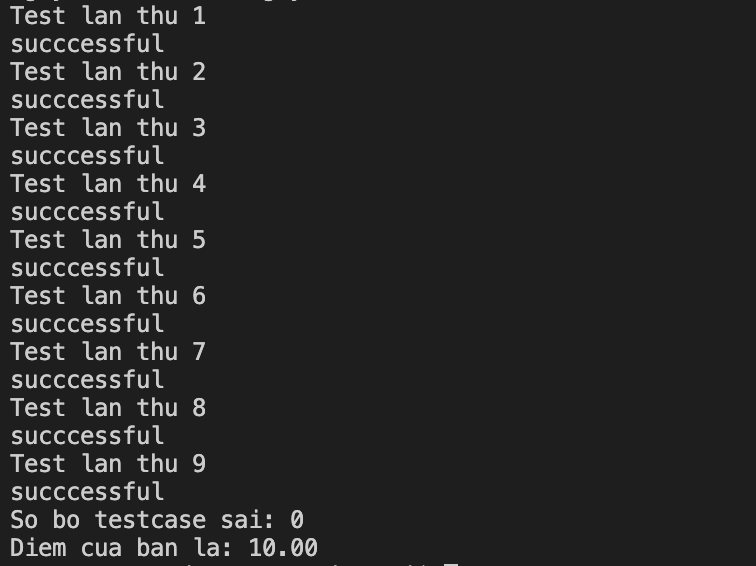
\includegraphics[scale=.3]{hinhanh/ketquademodung.png}
\end{center}
\end{figure}

Trong lần chấm điểm này bài tập của sinh viên đã đúng hết tất cả các bộ testcase của chương trình. Sau khi chạy hết tất cả các bộ test chương trình sẽ thông báo số bộ test không đúng của sinh viên là 0 và điểm số của sinh viên là 10.00đ.

\subsection{Bài tập với đầu vào là một mãng số nguyên có n phần tử}

Đề bài: Cho một mãng số nguyên có n phần tử. Sắp xếp mãng số nguyên đó theo thứ tự tăng dần.

Ví dụ: Nếu cho một mãng sau arr = [3, 1, 7, 10, 2, 14], sau khi được sắp xếp mãng số nguyên đó sẽ trở thành arr = [1, 2, 3, 7, 10, 14].

Trước khi đi vào chạy thực nghiệm, chúng ta sẽ đi qua tìm hiểu về cách tổ chức thư mục chứa các file dùng để thực thi khi tiến hành thực nghiệm.

\begin{figure}[ht]
\begin{center}
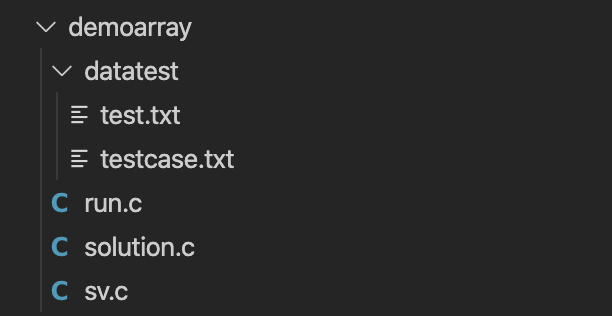
\includegraphics[scale=.3]{hinhanh/cautrucdemoarray.png}
\end{center}
\end{figure}

Tương tự như cấu trúc của bài tập ở phần trên, bên trong thư mục demoarray sẽ có 1 thư mục datatest chứa thông tin của các bộ testcase, file solution.c để chứa code bài giải cho đề bài ở trên, file sv.c chứa code bài làm của sinh viên sau khi nộp bài và file run.c là file dùng để chạy chương trình chấm điểm cho bài tập của sinh viên.

Trong thư mục datatest sẽ có 2 file test.txt và testcase.txt. Cũng như ở bài trên file testcase.txt sẽ chứa thông tin tổng số bộ test cần thực hiện và các bộ test cần thực hiện. Và mỗi lần kiểm tra bộ test, chương trình sẽ tiến hành ghi từng bộ test ra file test.txt.

Như hình bên dưới thì dòng đầu tiên sẽ biểu hiện tổng số bộ testcase. Các dòng tiếp theo sẽ là các bộ testcase. Ở trong file này cứ 2 dòng liên tiếp sẽ ứng với 1 bộ testcase với dòng đầu tiên ứng với số phần tử của mảng và dòng tiếp theo là các phần tử của mãng (các phần tử trong mãng được phân cách với nhau bằng dấu cách). Với mỗi lần thực hiện chương trình sẽ đọc thông tin ở 2 dòng liên tiếp (trừ dòng đầu tiên) để ghi sang file test.txt là cho mỗi lần chạy chương trình.

\begin{figure}[ht]
\begin{center}
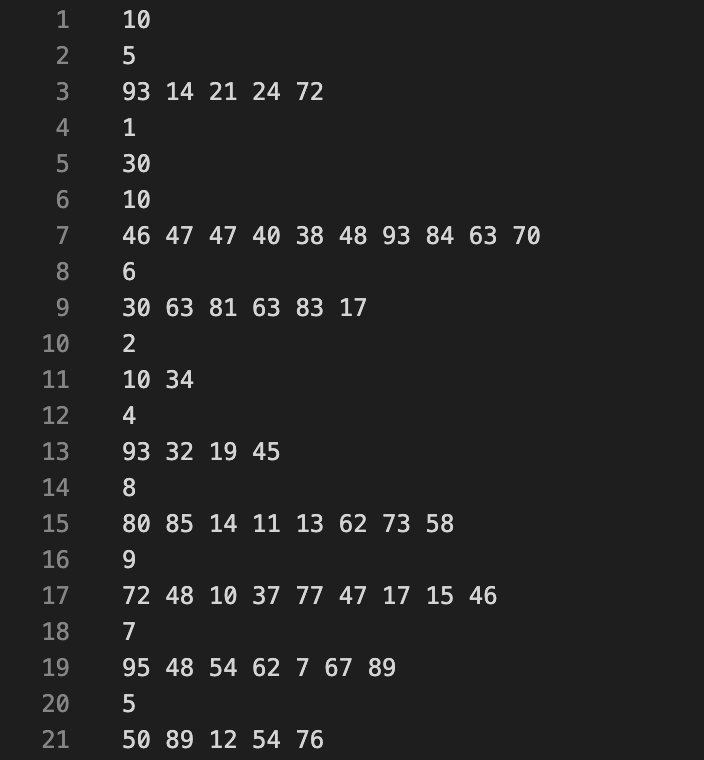
\includegraphics[scale=.3]{hinhanh/testcasearray.png}
\end{center}
\end{figure}

Để chạy thực nghiệm đối với bài toán trên, tôi sẽ tiến hành chạy thử ở hai trường hợp đó là một bài của sinh viên làm đúng và một bài của sinh viên làm chưa chính xác.

Đầu tiên tôi sẽ tiến hành chạy thử trường hợp chưa chính xác. Cùng xem qua cách giải quyết sau của sinh viên:

\begin{lstlisting}
void sapXep(int a[100], int n){
    int tg;
    for(int i = 0; i < n - 1; i++){
        for(int j = i + 1; j < n; j++){
            if(a[i] > a[j] + 6){
                tg = a[i];
                a[i] = a[j];
                a[j] = tg;        
            }
        }
    }
}
\end{lstlisting}

Trong bài tập này trước khi tiến hành đọc dữ liệu từ file chứa testcase để chấm điểm, chương trình sẽ chạy trước hàm setup() để sinh test ngẫu nhiên (với testcase là các mãng số nguyên với số phần tử ngẫu nhiên).

\begin{lstlisting}
void printRandoms(int lower, int upper, int count, FILE *out) 
{ 
    int i;
    fprintf(out,"%d\n",count);
    for (i = 0; i < count; i++) { 
        int num = (rand() % 
           (upper - lower + 1)) + lower; 
        fprintf(out,"%d ",num); 
    }
    fprintf(out,"\n"); 
} 

int randomNumber(int lower, int upper)
{
    int num = (rand() % (upper - lower + 1)) + lower; 
    return num;
}

void setup(int lower, int upper, int n, FILE *out)
{
    int count;
    fprintf(out,"%d\n",n);
    srand(time(0)); 
    for(int i = 0; i < n; i++)
    {
        count = randomNumber(0, 10);
        printRandoms(lower, upper, count, out);
    } 
    fclose(out);
}
\end{lstlisting}

Trong hàm setup() tham số n dùng để quy định số bộ testcase ta muốn tạo trước khi chạy chương trình. Tham số lower và upper dùng để quy định giá trị các phần tử trong mảng sẽ có giá trị trong khoảng đó (các phần tử sẽ lớn hơn hoặc bằng lower và nhỏ hơn hoặc bằng upper). Tham số out dùng để ghi các thông tin vào file, cụ thể ở đây là ghi số lượng bộ testcase và các bộ testcase được tạo ra. Bên trong hàm setup() tôi sử dụng hàm randomNumber() để sinh ngẫu nhiên số lượng phần tử của mãng và hàm printRandoms() dùng để sinh các mãng số nguyên và ghi vào trong file.

Cùng xem qua đoạn mã thực hiện chấm điểm sau:

\begin{lstlisting}
int main ()
{
    FILE *inp, *out, *outTestcase;
    int n, arr[100] , m, lower = 1, upper= 100, wrong, success;
    float diem;
    success = 0;
    wrong = 0;

    if((outTestcase = fopen("./datatest/testcase.txt", "w")) == NULL)
    {
        printf("Error! opening file");
        exit(1);         
    }
    setup(lower,upper, 10,outTestcase);
    if ((inp = fopen("./datatest/testcase.txt", "r")) == NULL)
    {
        printf("Error! opening file");
        exit(1);         
    }
    fscanf(inp,"%d",&n);

    for(int i = 0; i < n; i++) {
        if((out = fopen("./datatest/test.txt", "w")) == NULL)
        {
            printf("Error! opening file");
            exit(1);         
        }
        printf("Test lan thu %d\n", i + 1);

        fscanf(inp,"%d",&m);
       
        for(int i = 0; i < m; i++) {
            fscanf(inp,"%d", &arr[i]);
        }

        fprintf(out,"%d\n",m);
        for(int i = 0; i < m; i++) {
            fprintf(out,"%d ",arr[i]);
        }
        fclose(out);

        char commandSolution[50],commandRunSolution[50],commandSV[50];
        char commandRunSV[50],commandCompare[50];

        strcpy(commandSolution, "gcc -Wall -o solution solution.c" );
        strcpy(commandSV, "gcc -Wall -o sv sv.c" );
        strcpy(commandRunSolution, "./solution");
        strcpy(commandRunSV, "./sv");
        strcpy(commandCompare, "diff ./out.txt ./outsv.txt");
        system(commandSolution);
        system(commandSV);
        system(commandRunSolution);
        system(commandRunSV);

        if(system(commandCompare) == 0) {
            printf("succcessful\n");
            success = success + 1;
        }else {
            wrong = wrong + 1;
            printf("wrong\n");
            printf("Bo test case: ");
            for(int i = 0; i < m; i++) {
                printf("%3d", arr[i]);
            }
            printf("\n");
        }
    }
    fclose(inp);
    diem = (10.0 / n) * success;
    printf("So bo testcase sai: %d\n", wrong);
    printf("Diem cua ban la: %.2f\n", diem);
    return(0);
}
\end{lstlisting}

Như ở trên tôi tiến hành gọi hàm setup() để tạo trước các bộ testcase được ghi vào trong file testcase.txt.

Trong đoạn code trên tôi sử dụng hàm fopen() để đọc ghi file, tham số đầu tiền sẽ là đường dẫn đích đến file cần đọc/ghi, tham số thứ 2 dùng để truy cập đến chế độ cần sử dụng (đọc hoặc ghi file,...).

Ví dụ: hàm fopen("./datatest/testcase.txt", "r") sẽ tiến hành truy cập vào file testcase.txtđể đọc dữ liệu.

Sau khi dọc dữ liệu từ testcase.txt và ghi dữ liệu vào file test.txt chương trình sẽ thực thi các câu lệnh hệ thống để biên dịch các file có phần mở rộng là .c. Sau khi đã biên dịch xong sẽ sử dụng file output của quá trình biên dịch để chạy chương trình. Như ở trên thì tôi sử dụng hàm system() để có thể thực thi các lệnh hệ thống trong C.

Khi chạy xong các file biên dịch, chương trình sẽ cho ra 2 file output kết quả. Để biết là bài tập sinh viên có chạy đúng với bộ tetscase tương ứng hay không tôi sử dụng lệnh diff để kiểm tra sự khác biệt của 2 file output.

Sau khi đã tiến hành kiểm tra hết tất cả bộ testcase, chương tình sẽ tính được điểm của sinh viên dựa trên số bộ testcase đúng và số bộ testcase không đúng.

Cùng xem qua quá trình chạy thực nghiệm đối với đề bài ở trên:

Cũng như ở phần trên tôi sẽ tiến hành biên dịch file run.c trước khi chạy.

\begin{figure}[ht]
\begin{center}

\includegraphics[scale=.3]{hinhanh/compilerdemoarray.png}
\end{center}
\end{figure}

Sau khi compiler thành công trong thư mục sẽ xuất hiện thêm file run.

\begin{figure}[ht]
\begin{center}
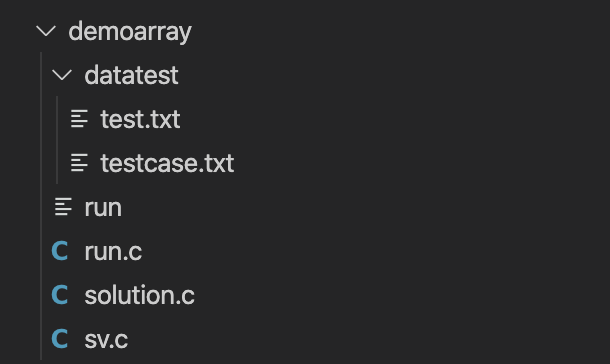
\includegraphics[scale=.3]{hinhanh/cautrucarraysaucompiler.png}
\end{center}
\end{figure}

Để có thể chạy chương trình chúng ta tiến hành chạy file run vừa được tạo ra.

\begin{figure}[ht]
\begin{center}

\includegraphics[scale=.3]{hinhanh/rundemoarray.png}
\end{center}
\end{figure}

Kết quả khi chạy file run để chấm điểm.

\begin{figure}[ht]
\begin{center}
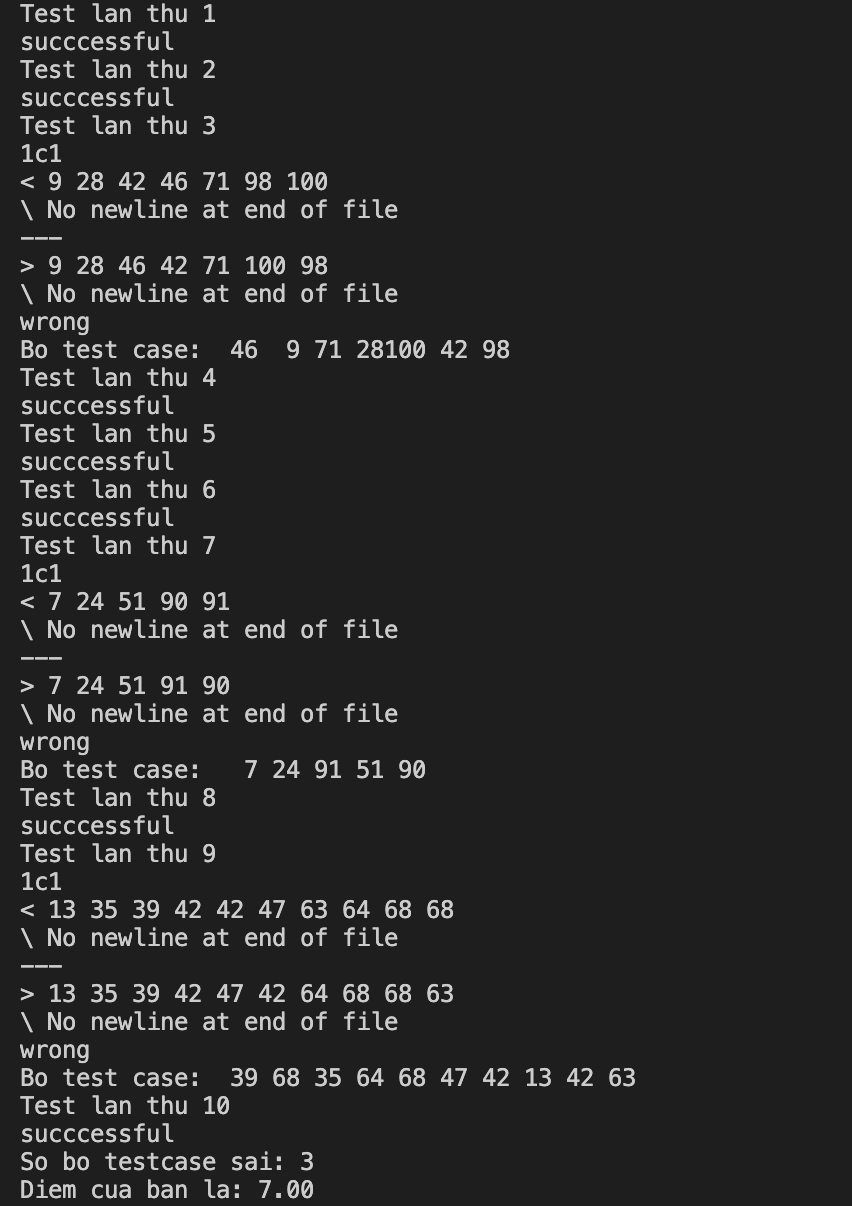
\includegraphics[scale=.3]{hinhanh/ketquademoarray.png}
\end{center}
\end{figure}

Như hình bên trên chúng ta thấy chương trình có tất cả 10 bộ test. Khi chạy thì chúng ta thấy được các bộ testcase ở lần thứ 3, 7, 9 sẽ thực hiện không chính xác. Ví dụ như ở bộ test thứ 3 với bộ testcase đầu vào là arr = [46, 9, 71, 28, 100, 42, 98] thì kết quả của solution cho ra là [9, 28, 42, 46, 71, 98, 100] còn của sinh viên cho ra kết quả là [9, 28, 46, 42, 71, 100, 98]. Như ta thấy được thì kết quả của solution cho ra là đúng như mong đợi còn kết quả của sinh viên cho ra là chưa chính xác. Sau khi chạy hết tất cả các bộ test chương chình sẽ thông báo số bộ test không đúng của sinh viên là 3 và điểm số của sinh viên là 7.00đ.

Cùng xem lại thư mục sau khi chạy xong file run.

\begin{figure}[ht]
\begin{center}
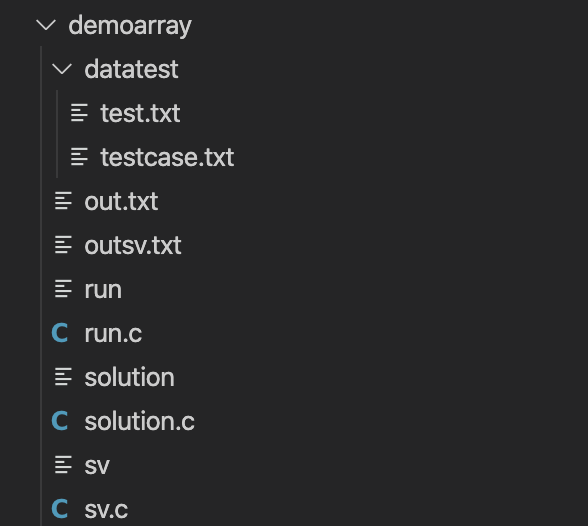
\includegraphics[scale=.3]{hinhanh/cautrucsauchayrunarray.png}
\end{center}
\end{figure}

Trong quá trình chạy chương trình sẽ sinh ra 2 file solution và sv sau quá trình compiler. Sau khi chạy 2 file soution và sv sẽ sinh ra 2 file output là out.txt và outsv.txt.

Tiếp theo tôi sẽ tiến hành chạy trường hợp thứ 2 đó là trường hợp bài làm của sinh viên cho ra kết quả chính xác. Cùng xem qua cách giải quyết sau:

\begin{lstlisting}
void sapXep(int a[100], int n){
    int tg;
    for(int i = 0; i < n - 1; i++){
        for(int j = i + 1; j < n; j++){
            if(a[i] > a[j]){
                tg = a[i];
                a[i] = a[j];
                a[j] = tg;        
            }
        }
    }
}
\end{lstlisting}

Cũng giống như trường hợp đầu tiên, tôi sẽ biên dịch file run.c bằng câu lệnh gcc -Wall -o run run.c để có được file biên dịch run. Sau đó để chạy được chương trình chúng ta tiến hành chạy file run được sinh ra. Sau đó chúng ta nhận được kết quả như sau.

\begin{figure}[ht]
\begin{center}
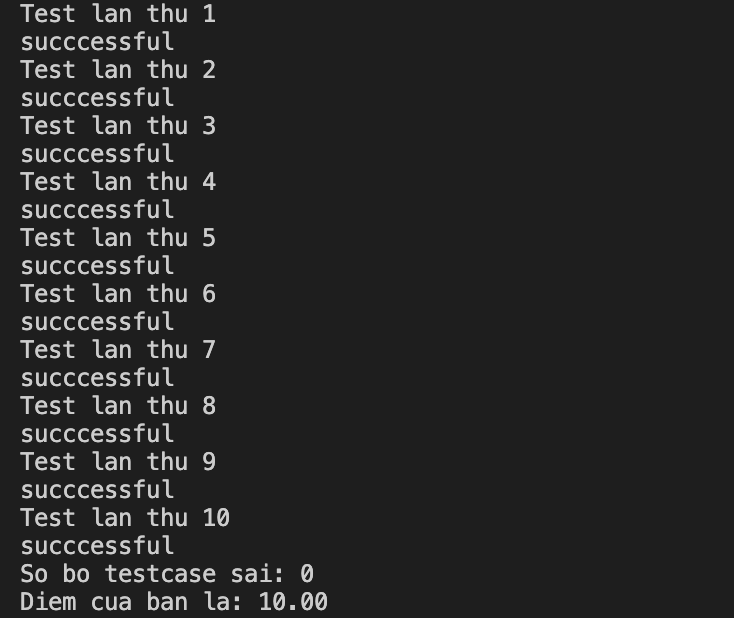
\includegraphics[scale=.3]{hinhanh/ketquademoarraydung.png}
\end{center}
\end{figure}

Trong lần chấm điểm này bài tập của sinh viên đã đúng hết tất cả các bộ testcase của chương trình. Sau khi chạy hết tất các các bộ tetscase chương trình sẽ thông báo số bộ testcase không đúng của sinh viên là 0 và điểm số của sinh viên là 10.00đ.

\bibliographystyle{plain}
\bibliography{tailieuthamkhao.bib}
\end{document}


